% !Mode:: "TeX:UTF-8"
%% !TEX program  = xelatex
%! TEX program = xelatex
%\documentclass{cumcmthesis}
\documentclass[withoutpreface,bwprint]{cumcmthesis} %去掉封面与编号页,电子版提交的时候使用。
\usepackage{etoolbox}
\BeforeBeginEnvironment{tabular}{\zihao{-5}}
\usepackage{cite}
\usepackage[numbers,sort&compress]{natbib}
\usepackage[framemethod=TikZ]{mdframed}
\usepackage{url}   % 网页链接
\usepackage{subcaption} % 子标题
\title{基于双层规划的鲜奶配送站点的最优化设置}
\tihao{A}
\baominghao{4321}
\schoolname{中国地质大学(武汉)}
\membera{ }
\memberb{ }
\memberc{ }
\supervisor{ }
\yearinput{2020}
\monthinput{08}
\dayinput{22}
\usepackage{yhmath}
\graphicspath{{figures/}}
\usepackage{graphicx} % 使用图形格式
\usepackage{epstopdf} % 将 EPS 转换为 PDF
\usepackage{enumerate}


\begin{document}
	
	\maketitle
	\begin{abstract}
		
		在现代社会,生鲜配送与人们的生活紧密相连,它不仅仅是商品的简单流通,更是满足消费者日常需求的重要环节。其中,鲜奶作为生鲜产品中的一大类,其配送的时效性和新鲜度更是备受关注。然而,在物流的“最后一公里”环节中,鲜奶配送往往面临着诸多挑战,如何合理设置鲜奶配送站点的位置和数量,成为了牛奶公司必须面对并解决的实际难题。
		
		\textbf{对于问题一,}本文通过量化配送距离、车辆数和建站数,运用\textbf{线性加权法}进行了\textbf{无量纲处理}。利用\textbf{K-means聚类算法}和\textbf{肘部法则}确定建站数量,对于聚类所得每一类,采用\textbf{双层规划方法}构建模型,得出每一簇中距离之和最短且成本较低的网点,将其作为配送站设置点。总而得到最优的鲜奶配送站设置方案。
		
		\textbf{对于问题二,}本文针对题述要求,在\textbf{最长10分钟配送时间}的限制下,寻求最小配送站建设成本的最优方案。本文先将时间限制转化为实际距离限制,将实际距离限制转变为\textbf{二维坐标图中}的距离限制。从而引入网点在配送站点最大配送距离内的限制条件,对双层规划模型中的上层规划进行改进。利用MATLAB,计算得出了在设定的配送时间限制下,建设成本最低的配送站点建设方案。
		
		
		\textbf{对于问题三,}鉴于题述中对于配送站点方案的需求,即均衡各鲜奶配送站的配送量,本文首先计算了所有配送网点的总订奶量,并进一步在确定了最优聚类数K的条件下,计算得出平均订奶量。随后,基于这一平均订奶量,设定一个配送量的\textbf{均衡区间[a,b]}。对聚类结果进行判断,对于不均衡的情况,更改簇边缘网点聚类位置,最终使所有配送站各自的配送量$p_{h}$均落在此\textbf{均衡区间[a,b]}内,即每个配送站的配送量已达到\textbf{均衡状态},这样既避免了资源的过度浪费,也确保了配送的及时性。而后改进问题二所建立的双层规划模型,在下层规划中,额外加入了鲜奶的配送成本作为考量因素,得到选定鲜奶配送站下鲜奶配送的最优路径。最终,通过\textbf{新的双层规划模型}得到新的最优鲜奶配送站的设置方案。		
		
		
		\keywords{二维图\quad  K-means聚类\quad  双层规划\quad 线性加权法\quad 不同约束条件下最优配送站点设置 \quad  }
	\end{abstract}
	
	%目录  2019 明确不要目录,我觉得这个规定太好了
	%\tableofcontents
	
	%\newpage
	
	\section{问题重述}
	\subsection{问题背景}
生鲜配送作为与民众日常生活紧密相连的重要环节,"最后一公里"的物流瓶颈问题尤为凸显。特别是对于鲜奶配送而言,时效性是其核心要素。鲜奶配送站每日清晨,必须运用非冷链小型物流车辆,确保当日鲜奶在第一时间准确、高效地送达至片区内的各个分销网点。因此,如何科学、合理地规划配送站点的布局与数量,已然成为牛奶公司亟待解决的实际问题。
	\subsection{问题要求}
	
	\textbf{问题1}  在配送时间尽量缩短的情况下,得到最经济的配送站点设置方案。
	
	\textbf{问题2}  在确保配送时效不超过10分钟的条件下,得出最小化建设成本的鲜奶配送站的最优设置方案。
	
	\textbf{问题3} 在配送量均衡的条件下,得出最小化配送成本和较高配送时效与效率的鲜奶配送站的最优设置方案。
	
	
	\section{问题分析}
	\subsection{问题一分析}
	\textbf{对于问题一,}需要在配送效率与配送时效较高条件下,最小化配送成本以得到鲜奶配送站的最优设置方案。
	
	首先,对问题一进行合理简化,将各个抽象概念转化为具体可量化的指标。如用网点间的距离指代配送速度,用配送车辆数指代配送成本,用配送中心建站数指代建设成本。从而能够衡量各因素对配送站点设置方案的影响。
	
	同时,对经济成本与配送距离对方案设置的影响权重进行深入分析,确定两者各自的占比,再进行无量纲处理。随后,利用K-means聚类算法,根据网点分布的密集程度进行聚类,根据肘部法则以确定合适的建站数量。完成聚类后,计算同一分区中各个网点到其余网点的距离之和,将每个分区中距离之和最短的网点作为配送站点。最后,运用双层规划方法,制定出在配送速度和配送成本、建设成本上均达到优化目标的鲜奶配送站设置方案。
	
	\subsection{问题二分析}	
	\textbf{对于问题二}需要在配送时间为10分钟以内的条件下,考虑最小的配送站建设成本,得到最优的配送站点设置方案。
	其等同于在问题一基础上增加一个限制:配送站点的配送最大配送距离为S,即对双层规划中上层规划的目标函数增加了额外的约束条件,其为网点在配送站的配送范围内,其公式表达式为:$D_{ij}\le d,i\in I,j\in J$。 由运动学公式S=vt ,求出配送站的配送最大配送距离为S,依照附录所给图上距离与实际距离的比例尺求出d的大小。即可完成对问题一所建模型的改进与优化,从而得到解决问题二的数学模型。依照所建立模型利用Matlab计算得到在题设的配送时间限制下,建设成本最低的配送站点建设方案。
	
	\subsection{问题三分析}
	\textbf{对于问题三,}题述要求需要保证配送站点方案中各鲜奶配送站的配送量均衡。因此,本文首先计算了所有网点的总订奶量,以及最优聚类数K下的平均订奶量,并依据平均订奶量设置配送量的均衡区间[a,b]。若所有配送站各自的配送量$p_{h}$在此均衡区间[a,b]内,则可判定每个配送站的配送量均衡,既不造成资源浪费,也不延误配送。
	根据上述分析,本文基于问题二所建立数学模型的基础上,在进行双层规划寻找最优配送站设置方案前,建立了一个新的目标函数:$a\le p_{h}\le b$,并规划其约束条件,使得每一簇中设置的配送站配送量均衡,同时本文优化问题二的双层规划模型,于下层规划中额外考虑鲜奶的配送成本以得到最佳配送路径。从而得到配送量均衡的新鲜奶配送站的设置方案。
	

	
	\section{模型假设}
	
	\begin{itemize}
		\item 题述网点中,两两网点间或配送站与网点间的道路均为直线。
		\item 每个鲜奶配送站都有足够的非冷链小型物流车,且配送站的规模容量可以满足网点订奶量。
		\item 一个网点有且仅由一个鲜奶配送站供应。
		\item 每辆非冷链小型物流车的时速恒定不变,不受道路车流量影响。
	\end{itemize}
	
	\section{符号说明}
	% Table generated by Excel2LaTeX from sheet 'Sheet1'
	


\begin{table}[H]
	\centering
	\renewcommand{\arraystretch}{1.1}
	\setlength{\tabcolsep}{38pt}  % 增加列间距
	\caption{符号说明1}
	\begin{tabular}{ccl}
		\toprule
		集合    &说明    \\
		\midrule
		$I$ & 该市网点集合,I =\{1,2,..., 92\}\\
		$J$ & 候选配送站集合,J =\{1,2, ...,92\} \\
		$N$ & 配送车辆集合   N=\{1,2,...,n\}\\
		$I_k$&聚类后每一簇中的网点集合$I_k$=\{1,2,3,...,f\}\\
		\bottomrule
	\end{tabular}
	\label{tab:符号说明1}
\end{table}
\begin{table}[H]
	\centering
	\renewcommand{\arraystretch}{1.1}
	\setlength{\tabcolsep}{21pt}  % 增加列间距
	\caption{符号说明2}
	\begin{tabular}{ccc} 
		\toprule
		变量    & 取值范围 & 说明 \\
		\midrule
		$h_j$       &\{0,1\}  & 判断是否选择 j 点建设配送站。 \\
		$z_{ij}$    &\{0,1\}  &判断是否选择配送站j作为网点i的配送点 \\
		$y_{ijn}$   &\{0,1\}  &判断车辆n是否从配送站j出发为网点i配送鲜奶\\
		$\omega _i$ &\{$Z_+$\}&网点i的订奶量\\
		$r_{ij}$    &\{$Z_+$\}&配送站j配送鲜奶到网点i的单位成本\\
		$D_{ij}$    &\{$Z_+$\}&配送站j到网点i的距离\\
		$C_{nj}$    &\{$R_+$\}&配送站j派遣车辆n的单位时间成本\\
		$C_n$       &\{$R_+$\}&车辆n的自身成本\\
		$C_j$		&\{$R_+$\}&单个配送站的建设成本\\
		$T$         &\{$R_+$\}&单个车辆从网点i到配送点j的行驶时间\\
		\bottomrule
	\end{tabular}
	\label{tab:符号说明}
\end{table}
	
	
	% \usepackage{booktabs}
	
	
% \usepackage{booktabs}



	
	
	\section{问题一模型的建立和求解}
	\subsection{模型建立}


	\subsubsection{数据可视化}
	根据所给附录数据,绘制题述片区中网点及网点间道路的二维坐标图。
	\subsubsection{K-means聚类确定配送站建站个数}
	\textbf{Step1: K-means聚类}
	对于题述片区中网点及网点间道路的二维坐标图,需要确定配送站的设置个数。针对这一问题,本文采用K-means聚类。
	
	K-means聚类是随机从数据集中选取K个点作为初始聚类中心,然后计算各个样本到聚类中心的距离,通过距离大小把样本归到离它最近的聚类中心所在的类。计算新形成的每个聚类的数据对象的平均值来得到新的聚类中心,调整到相邻两次的聚类中心没有任何变化为止。
	
	\textbf{Step2: 肘部法判断选取最佳聚类簇 K }
	
	对于最佳聚类簇 K 的选取方法,常用肘部法判断。肘部法利用观察 K 与 SSE的变化获得,SSE 随着 K 的增大而减小,并且在达到第一个临界转折点处,SSE减小速度变缓,这个临界转折点就可以考虑为最佳聚类性能的点,该点对应的 K就是最佳聚类数。
	
	\textbf{Step3: 判断聚类结果是否收敛}
	
	同时,在 K-means 算法中,每一轮迭代完成后,都需要判断聚类结果是否收敛。为此,在此定义一个目标函数,即差平方和函数(Sum of the Squared Error),定义如下:
	\begin{align*}
		SSE=\sum_{i=1}^{k}{\sum_{x \in {{C}_{i}}}^{}{d(x,{{c}_{i}}{{)}^{2}}}}
	\end{align*}
	
	其中,$x$是集合$D$的对象,$C_{i}$代表第i个簇,$c_{i}$是$C_{i}$的中心,${C_i} = \dfrac{1}{{{m_i}}}\sum\limits_{x \in {C_i}} x $, $m_{i}$是中心数据对象的个数。K-means算法迭代执行过程中,$SSE$ 的值会不断减小。当前后两轮迭代所得到的$SSE$保持不变或者二者之间的差异小于某个预设的门限值ε,就可以认为聚类结果已收敛。
	
	\subsubsection{采用双层规划寻找最优鲜奶配送站的设置方案}
	在确定鲜奶配送站的建站个数后,仍需要考虑K-means聚类后每一簇中鲜奶配送站的建站位置。从而得到最优的鲜奶配送站设置方案。
	
	针对这一问题,本文采用双层规划区寻找最优的鲜奶配送站的设置方案,双层规划在决策过程中,同时考虑两个不同层次或两个不同方面的规划或策略,从而很好地考虑到上层决策者和下层执行者之间的关系,进行规划。在此, 对于聚类后的每一簇,定义$I$为网点集合,$I=\{0,1,2, ... ,92\}$ , $J$为候选配送站集合, 有$J=\{1,2, ... , 92\}$ ,  $N$为配送车辆集合,$N=\{1,2, ... , n\}$
	
	为了寻找最优鲜奶配送站设置方案,设计双层规划流程图如图\ref{fig:双层规划流程图}所示:
	\begin{figure}[htbp]
		\centering
		\includegraphics[width=0.4\linewidth]{framework.pdf}
		\caption{双层规划流程图}
		\label{fig:双层规划流程图}
	\end{figure}
%	\newpage

\textbf{Step1: 建立上层规划模型}
	
\textbf{上层规划模型:}用于确定配送中心最优选址。题述中,鲜奶配送站应做到在配送在途时间尽可能短的同时最经济地配送鲜奶。
	
据此可以得到目标函数应由鲜奶配送站的总建设成本、配送点与各网点间的距离之和,以及鲜奶配送成本三者之和组成,并且应取其最小值,则目标函数为:
    
\begin{equation}
	{\rm{min }}{F_u} = \sum\limits_{j \in J}^{} {{C_j}} {h_j} + \sum\limits_{i \in I}^{} {\sum\limits_{j \in J}^{} {{D_{ij}}} } {z_{ij}}
	\label{eq:up}
\end{equation}

式\eqref{eq:up}中,其中${{C}_{j}}$为一个配送站的建设成本,${{h}_{j}}=\left \{{\begin{matrix}0,&j\text{点非配送点}\\&\\1,&\text{选择j点为配送点}\end{matrix}}\right .$,
${{D}_{ij}} \in {{Z}^{+}}$,示网点 i 与配送站 j 之间的距离,${{z}_{ij}}=\left \{{\begin{matrix}0,&\text{网点i非配送站j配送}\\&\\1,&\text{网点i有配送站j配送}\end{matrix}}\right .$,
${{\omega}_{i}}$表示网点i的订奶量,${{r}_{ij}}$表示网点i与配送站j之间配送鲜奶的单位成本。

式\eqref{eq:up}中,第一项$\sum\limits_{j\in J}^{}{{{C}_{j}}}{{h}_{j}}$表示总建设成本,第二项$\sum\limits_{i\in I}^{}{\sum\limits_{j\in J}^{}{{{D}_{ij}}}}{{z}_{ij}}$表示配送点与各网点间的距离。

目标函数的约束条件为:

\begin{equation}
	s.t.\left\{ {\begin{array}{*{20}{c}}
			{\sum\limits_{j \in J}^{} {{z_{ij}}}  = 1,}&{}&{i \in I}&{}\\
			{}&{}&{}&{}\\
			{{z_{ij}} \le {h_j},}&{}&{i \in I}&{j \in J}\\
			{}&{}&{}&{}\\
			{\sum\limits_{j \in J}^{} {{h_j} = K} }&{}&{}&{}\\
			{}&{}&{}&{}\\
			{{z_{ij}},{h_j} \in \{ 0,1\} ,}&{}&{i \in I}&{j \in J}
	\end{array}} \right.
\end{equation}

其中 ,$\sum\limits_{j \in J}^{} {{z_{ij}}}=1$表示每个网点有且仅有一个配送站服务;${z_{ij}} \le {h_j}$表示只有建设的配送站才可以提供服务;$\sum\limits_{j \in J}^{} {{h_j} = K} $表示建设的配送站数量为$K$ ;${{z}_{ij}}\in {{h}_{j}}$ 表示条件满足的状态。$K$为K-means聚类的最佳聚类数。

\textbf{Step2: 建立下层规划模型}

\textbf{下层规划模型}:用于确定鲜奶最佳配送路径,即行驶最短行程、使用最少时间、花费最低成本完成鲜奶配送任务。

据此可以得到目标函数应由车辆的配送成本和车辆的固定使用成本之和组成,并且应取其最小值,则目标函数为:
	\begin{equation}
		{\rm{min }}{F_2} = \sum\limits_{j \in J}^{} {T{C_{nj}}} {h_j} + \sum\limits_{j \in J}^{} {n{C_n}} {h_j}
	\end{equation}
	

式中,$T=\dfrac{{{D}_{ij}}}{V}$表示单个车辆从网点$i$到配送点$j$的行驶时间,${{C}_{nj}}$表示配送站$j$所派的配送车辆$n$单位时间内所消耗的成本,$n$表示配送站$j$使用的总非冷链小型物流车车辆数,$C_n$表示车辆$n$的固定使用成本。$\sum\limits_{j \in J}^{} {T{C_{nj}}} {h_j}$表示车辆的配送成本,$\sum\limits_{j \in J}^{} {n{C_n}} {h_j}$表示车辆的固定使用成本。


其约束条件为:
	\begin{equation}
s.t.\left \{{\begin{matrix}\sum_{i\in I}^{}{\sum_{n\in N}^{}{{{y}_{jin}}}}-{{h}_{j}}\le 0,&&i\in I&j\in J\\&&&\\\sum_{n\in N}^{}{{{y}_{ijn}}}\le 1,&&i\in I&j\in J\\&&&\\\sum_{n\in N}^{}{{{w}_{n}}}=N-1&&&\\&&&\end{matrix}}\right .
	\end{equation}

式中,${y_{ijn}} = \left\{ {\begin{array}{*{20}{c}}
			{1,}&{\text{车辆n从配送站j出发为网点i配送鲜奶}}\\
			{}&{}\\
			{0,}&{\text{车辆n不从配送站j出发}}
	\end{array}} \right.$。
	

$\sum\limits_{i \in I}^{} {\sum\limits_{n \in N}^{} {{y_{jin}}} }  - {h_j} \ge 0$表示非冷链小型运输车均是从鲜奶配送站派出的,$\sum\limits_{i \in I}^{} {\sum\limits_{n \in N}^{} {{y_{jin}}} }  - {h_j} \le 0$保证所有网点均有车辆配送货物;$\sum\limits_{n \in N}^{} {{w_n}}  = N - 1$保证每个网点只能出现在一台配送车辆的配送路径上;$\sum\limits_{i \in {w_n}}^{} {{q_{ni}}}  \le {Q_n}$保证每辆配送的鲜奶总量都小于该车的最大容量。
	 
在双层规划进行求解前,仍需考虑上下层各自目标函数的不可公度性,对目标函数进行预处理。
	 
\subsubsection{采用线性加权法对目标函数进行无量纲化处理}
本文采用线性加权法对目标函数进行无量纲化处理。线性加权法是根据目标的重要性确定一个权,以目标函数的加权平均值为评价函数,使其达到最优。线性加权法关键是要确定每个目标的权重,它反映不同目标在决策者心中的重要程度,重要程度高的权重就大,重要程度低的权重就小。相较于$\varepsilon$约束法、理想点法等方法更为简便、快捷。

该方法的基本步骤如下:
	
	\textbf{Step 1: 确定每个目标的权系数}
	
	\begin{align*}
		\begin{array}{l}
			\sum\limits_{j = 1}^m {{w_j}}  = 1.\\
			0 \le {w_j} \le 1,\\
			j = 1,2,3,...,m.
		\end{array}
	\end{align*}
	
	式中,$w_j$为各目标的权系数。
	
	\textbf{Step 2: 写出评价函数}
	\begin{align*}
		\sum\limits_{j = 1}^m {{w_j}{f_j}} (x)
	\end{align*}
	
	\textbf{Step 3: 求评价函数最优值}
	\begin{align*}
		{\rm{min }}\sum\limits_{j = 1}^m {{w_j}{f_j}} (x),\\
		s.t.x \in \Omega 
	\end{align*}
	
上述步骤中,$m$表示目标函数中子目标的个数,$f_j$指代子目标函数,$w_j$表示子目标函数的权系数,$x$表示决策变量,$ \Omega $ 表示可行域。

	\iffalse
	会报错
	\begin{enumerate}[Step 1:]
		\item 确定每个目标的权系数
	\end{enumerate}
	\begin{enumerate}[Step 2:]
		\item 写出评价函数
	\end{enumerate}
	\begin{enumerate}[Step 3:]
		\item 求评价函数最优值
	\end{enumerate}
	\fi
本文第一问建立的模型中,上层规划中,建设成本与最短配送距离的数量级差距较小,无需进行归一化处理,但两者的量纲不同,应用线性加权法进行无量纲处理。
	
	本文对于成本与距离的两个子目标的的期望权重均取0.5,则上层规划的目标函数变换如下:
	\begin{align*}
		{\rm{min }}{F_u} = 0.5\sum\limits_{j \in J}^{} {{C_{j}}} {h_j} + 0.5\sum\limits_{i \in I}^{} {\sum\limits_{j \in J}^{} {{D_{ij}}} } {z_{ij}}
	\end{align*}
	
	下层规划中数据的量纲一致且数量级相差不大,仍为:
	
	\begin{align*}
		{\rm{min }}{F_2} = \sum\limits_{j \in J}^{} {T{C_{nj}}} {h_j} + \sum\limits_{j \in J}^{} {n{C_n}} {h_j}
	\end{align*}
	
	\subsection{模型求解}
	\subsubsection{数据可视化}

\textbf{Step 1: }导入附录数据,列出各网点及连接道路的二维坐标图,如\ref{fig:二维坐标图}所示:
	\begin{figure}[htbp]
		\centering
		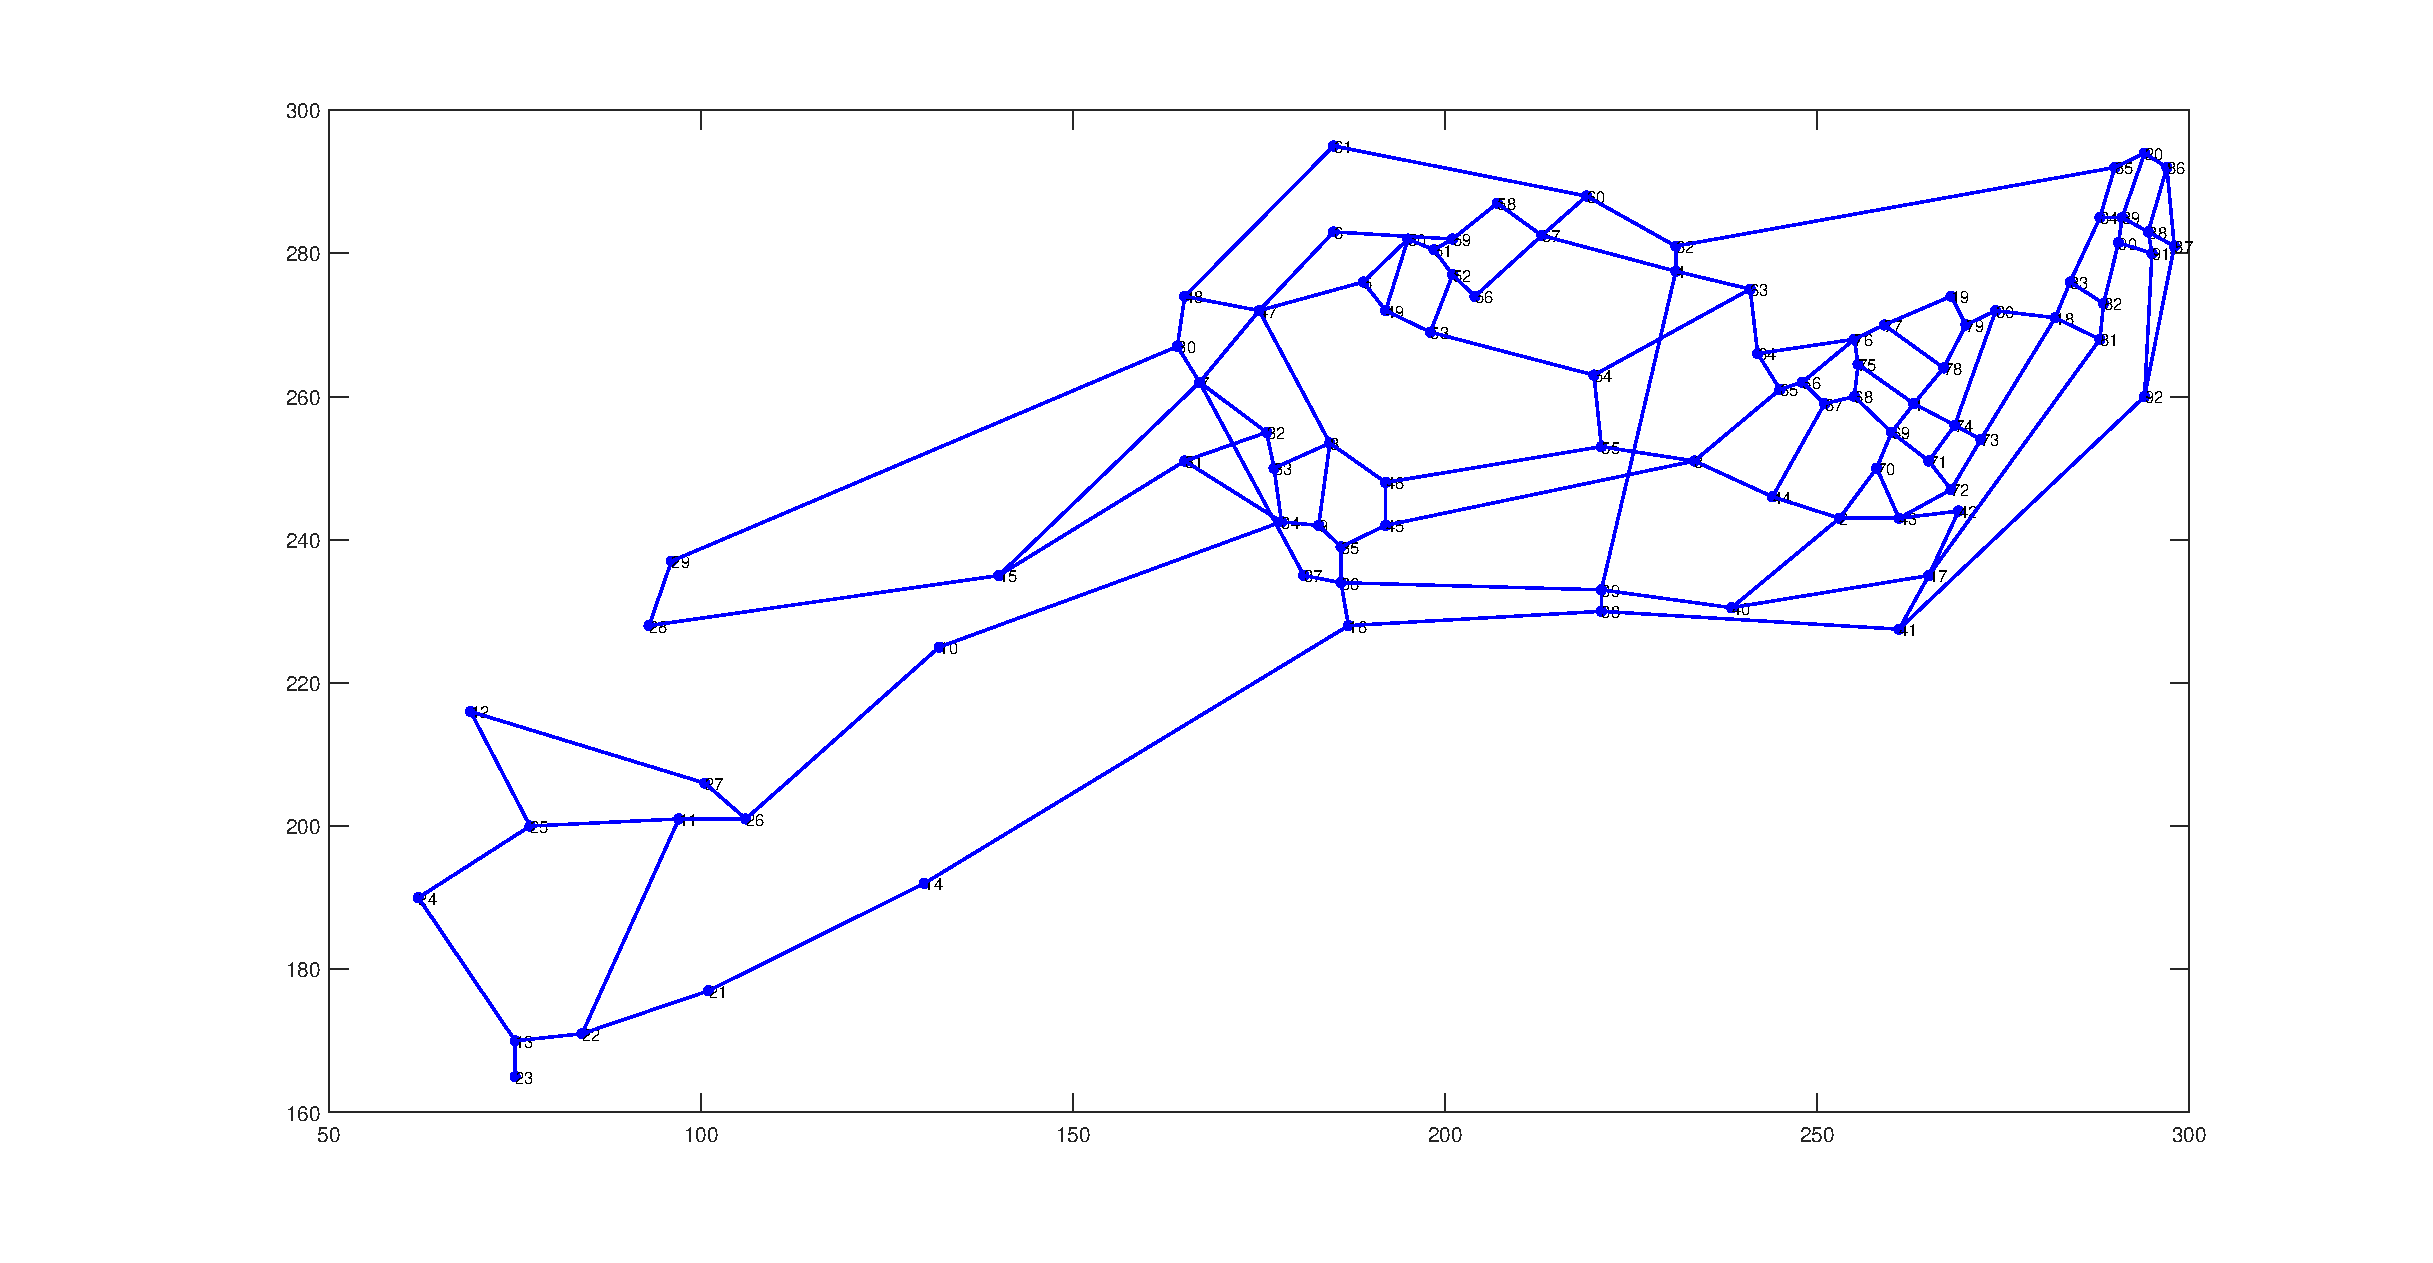
\includegraphics[width=16cm]{raw_real_G.eps}
		\caption{二维坐标图}
		\label{fig:二维坐标图}
	\end{figure}

\textbf{Step 2: }基于欧氏距离$D=\sqrt{{{(\Delta  x)}^{2}}+{{(\Delta  y)}^{2}}}$,计算得出各网点间道路的权重(距离)。

使用起始网点和终止网点分别为顶点对组$x$,$y$,再基于权重向量$D$构建赋权无向图,如图\ref{fig:赋权无向图}所示:
	\begin{figure}[htbp]
		\centering
		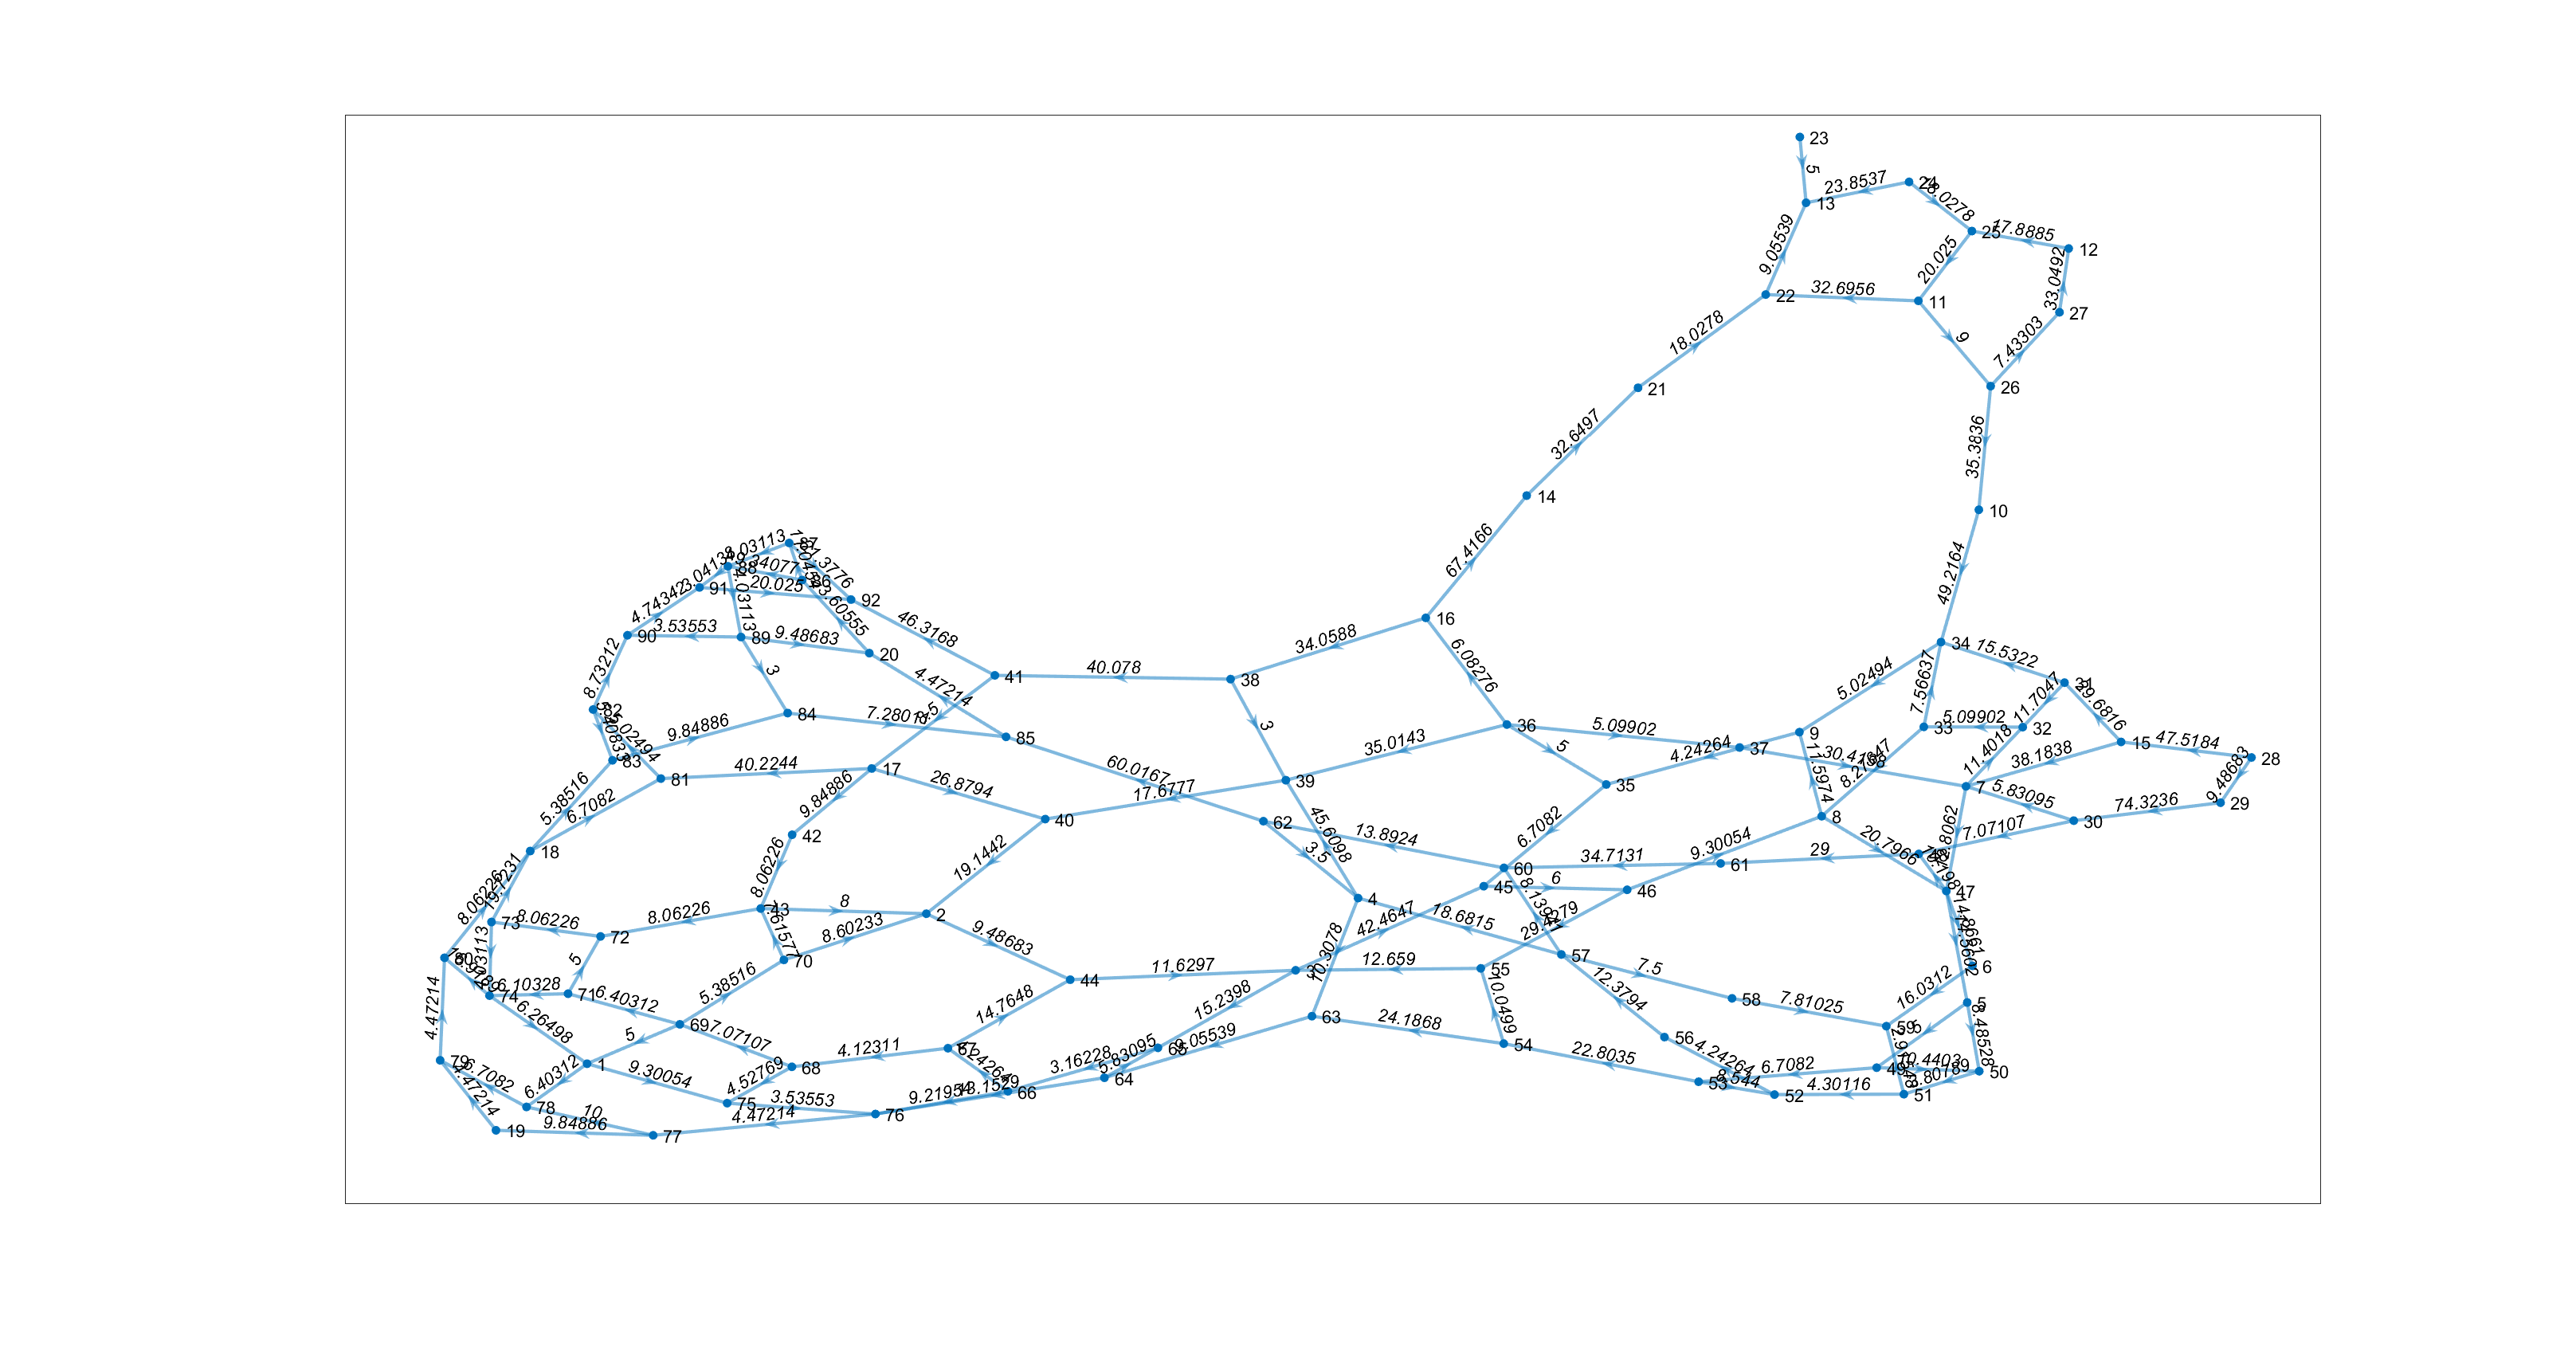
\includegraphics[width=16cm]{raw_G.eps}
		\caption{赋权无向图}
		\label{fig:赋权无向图}
	\end{figure}
	
\subsubsection{K-means 聚类模型求解}
	\textbf{Step 1: 绘制$SSE$与$K$的线性关系图}
	
$SSE$与$K$的线性关系如图\ref{fig:SSE与K线性关系图}所示,得到聚类结果收敛效果最好的聚类数从而确定建站个数。
	\begin{figure}[h]
		\centering
		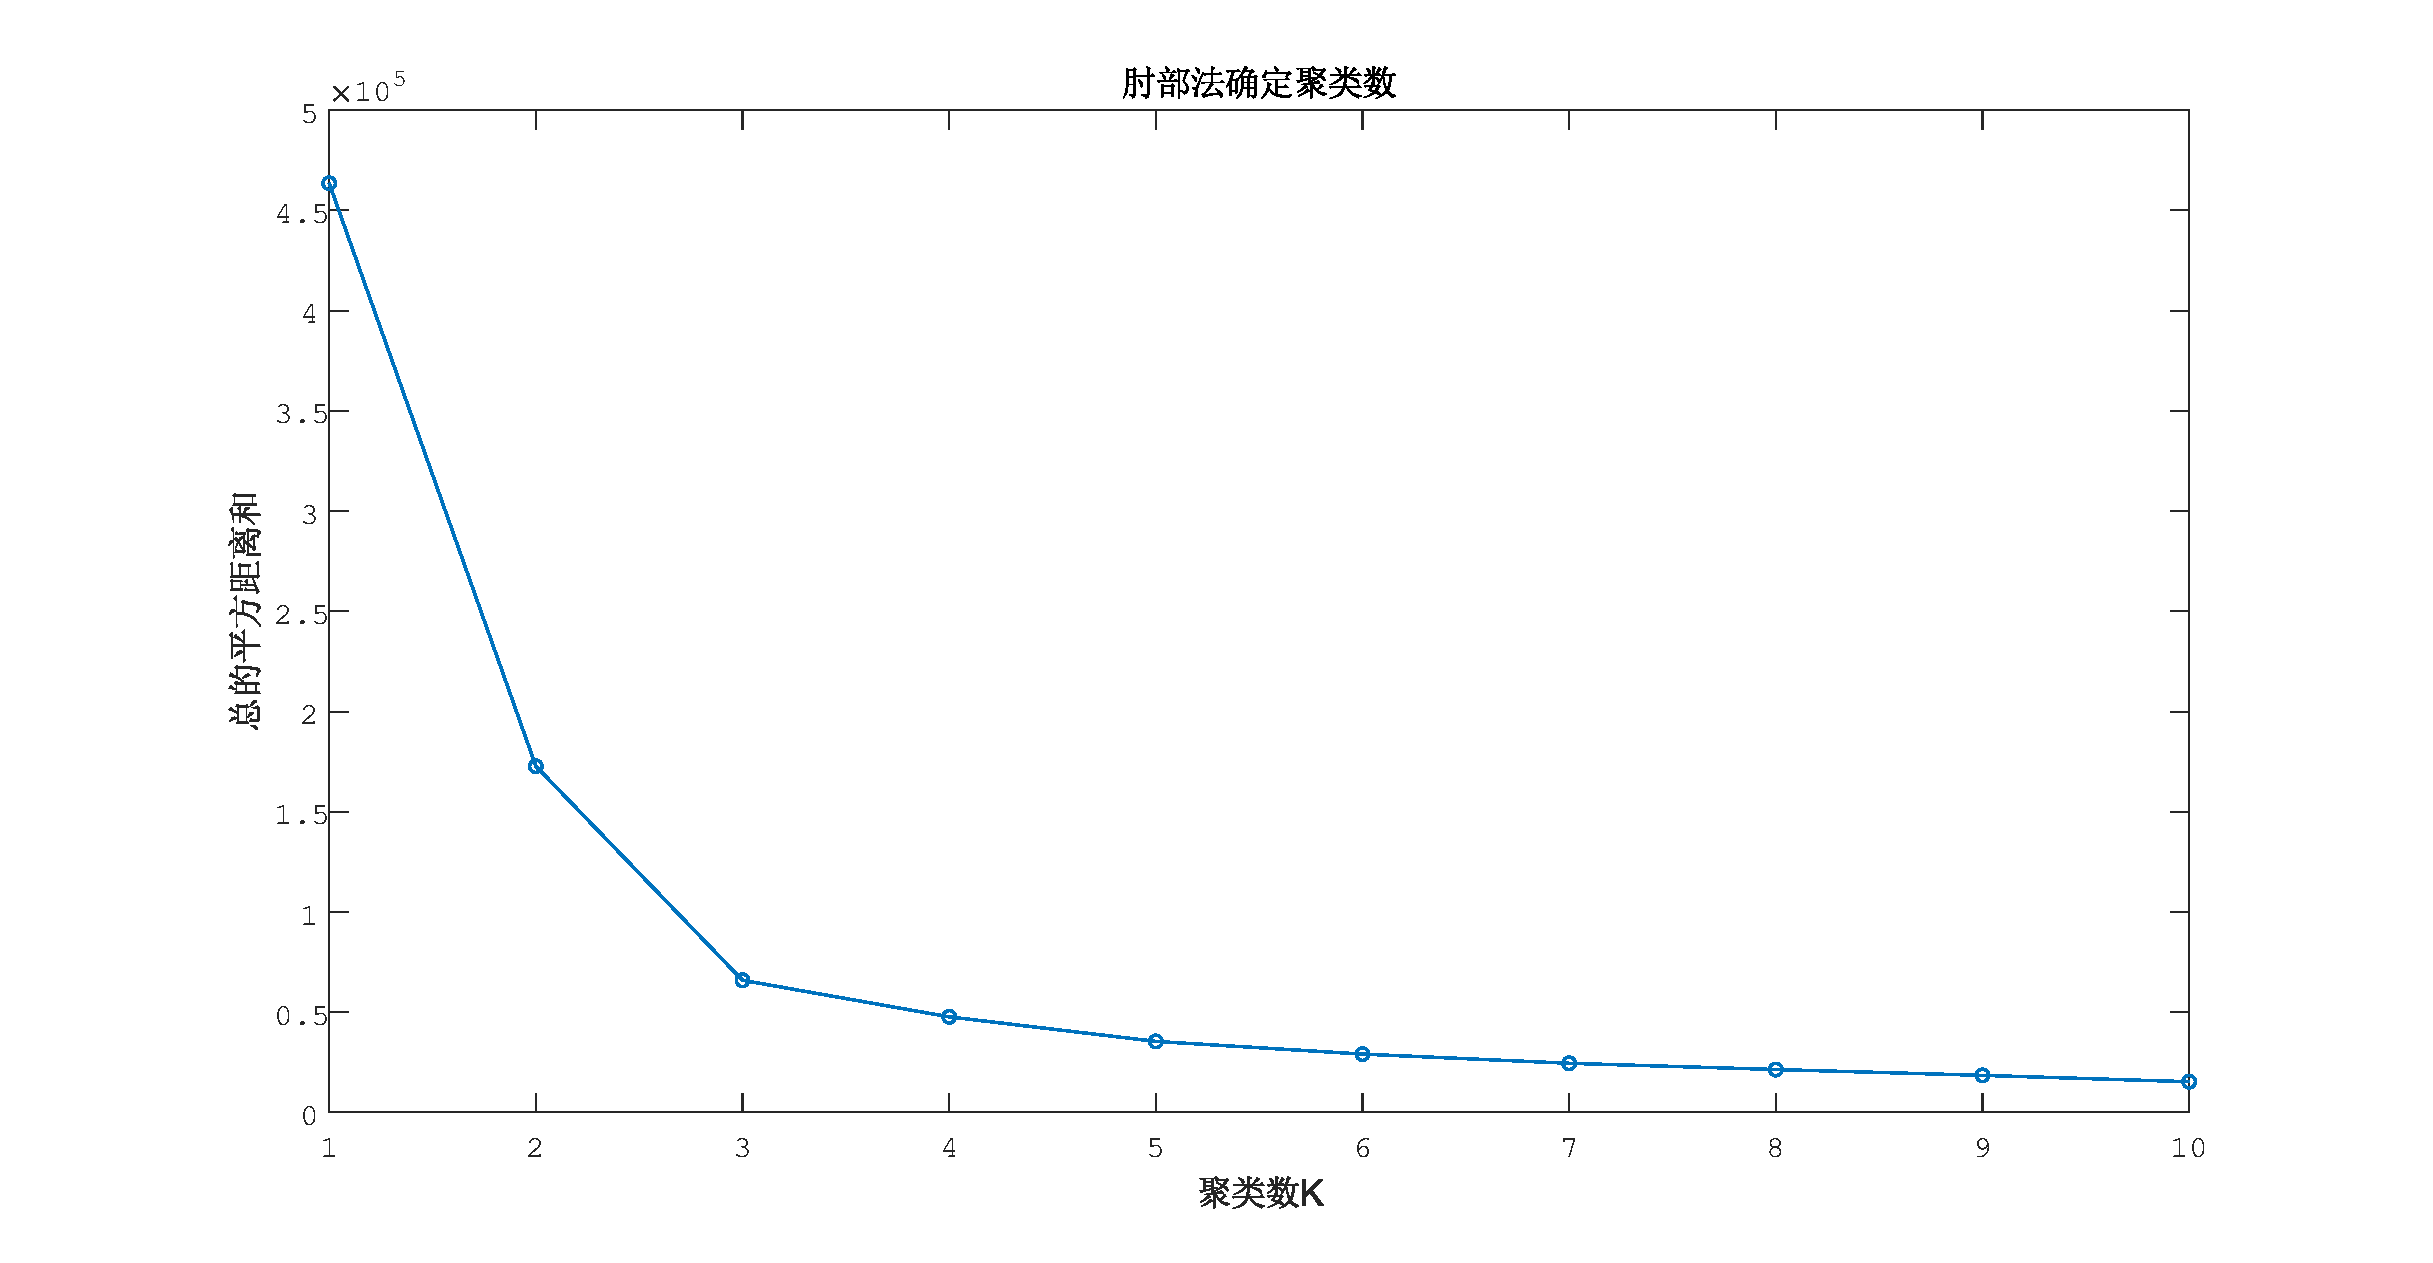
\includegraphics[width=13cm]{elbow.eps}
		\caption{SSE与K线性关系图}
		\label{fig:SSE与K线性关系图}
	\end{figure}
	
\textbf{Step2: 通过肘部法则得到最佳聚类数}

由肘部法则易得K=3为最佳聚类数,即建站个数为3,把样本归到离它最近的聚类中心所在的类,得出K-means聚类结果图\ref{K-means聚类结果图}所示:
	
	\begin{figure}[htbp]
		\centering
		\includegraphics[width=13cm]{kmeans.eps}
		\caption{K-means聚类结果图}
		\label{K-means聚类结果图}
	\end{figure}
	
	\textbf{Step3: 合理调整不连通网点}
	
在使用K-means方法简单聚类后注意到,得到的第三个聚类之间的部分网点并不直接连通,出于符合实际情境以及便于后续解题,手动将不连通的网点归于第二类,得从而到最终的聚类结果,修改后K-means聚类结果图如图\ref{fig:K-means聚类结果图(修改后)}所示:
	
	\begin{figure}[htbp]
		\centering
		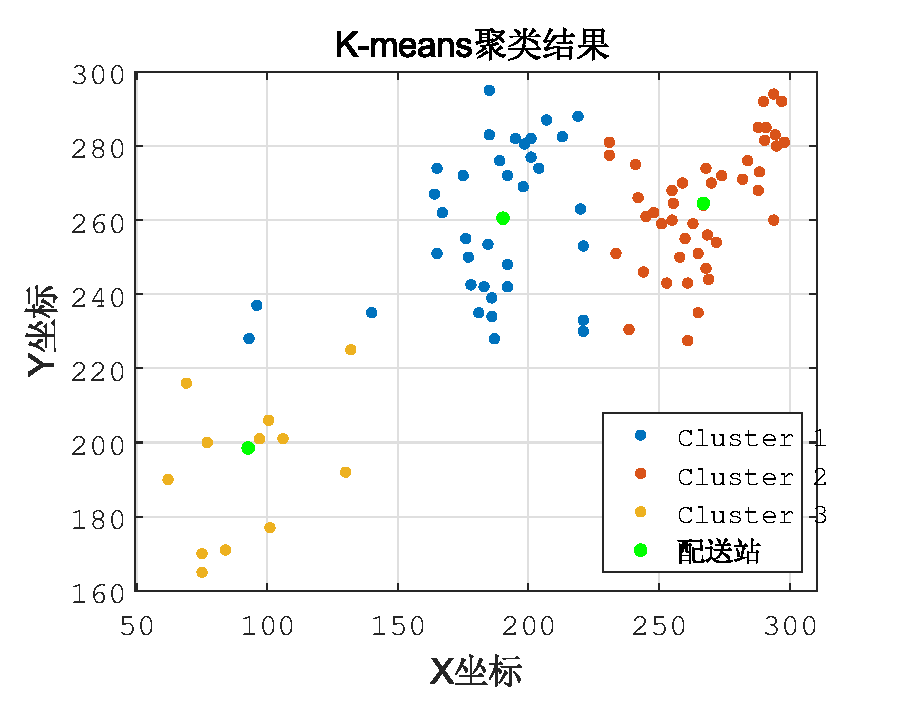
\includegraphics[width=13cm]{kmeans_re.eps}
		\caption{K-means聚类结果图(修改后)}
		\label{fig:K-means聚类结果图(修改后)}
	\end{figure}
	
	\textbf{Step4: 对每一簇构建赋权无向图}
	
	聚类后每一簇单独由网点对组x,y和权重向量D构建赋权无向图:
	
	\begin{figure}[htbp]
		\centering
		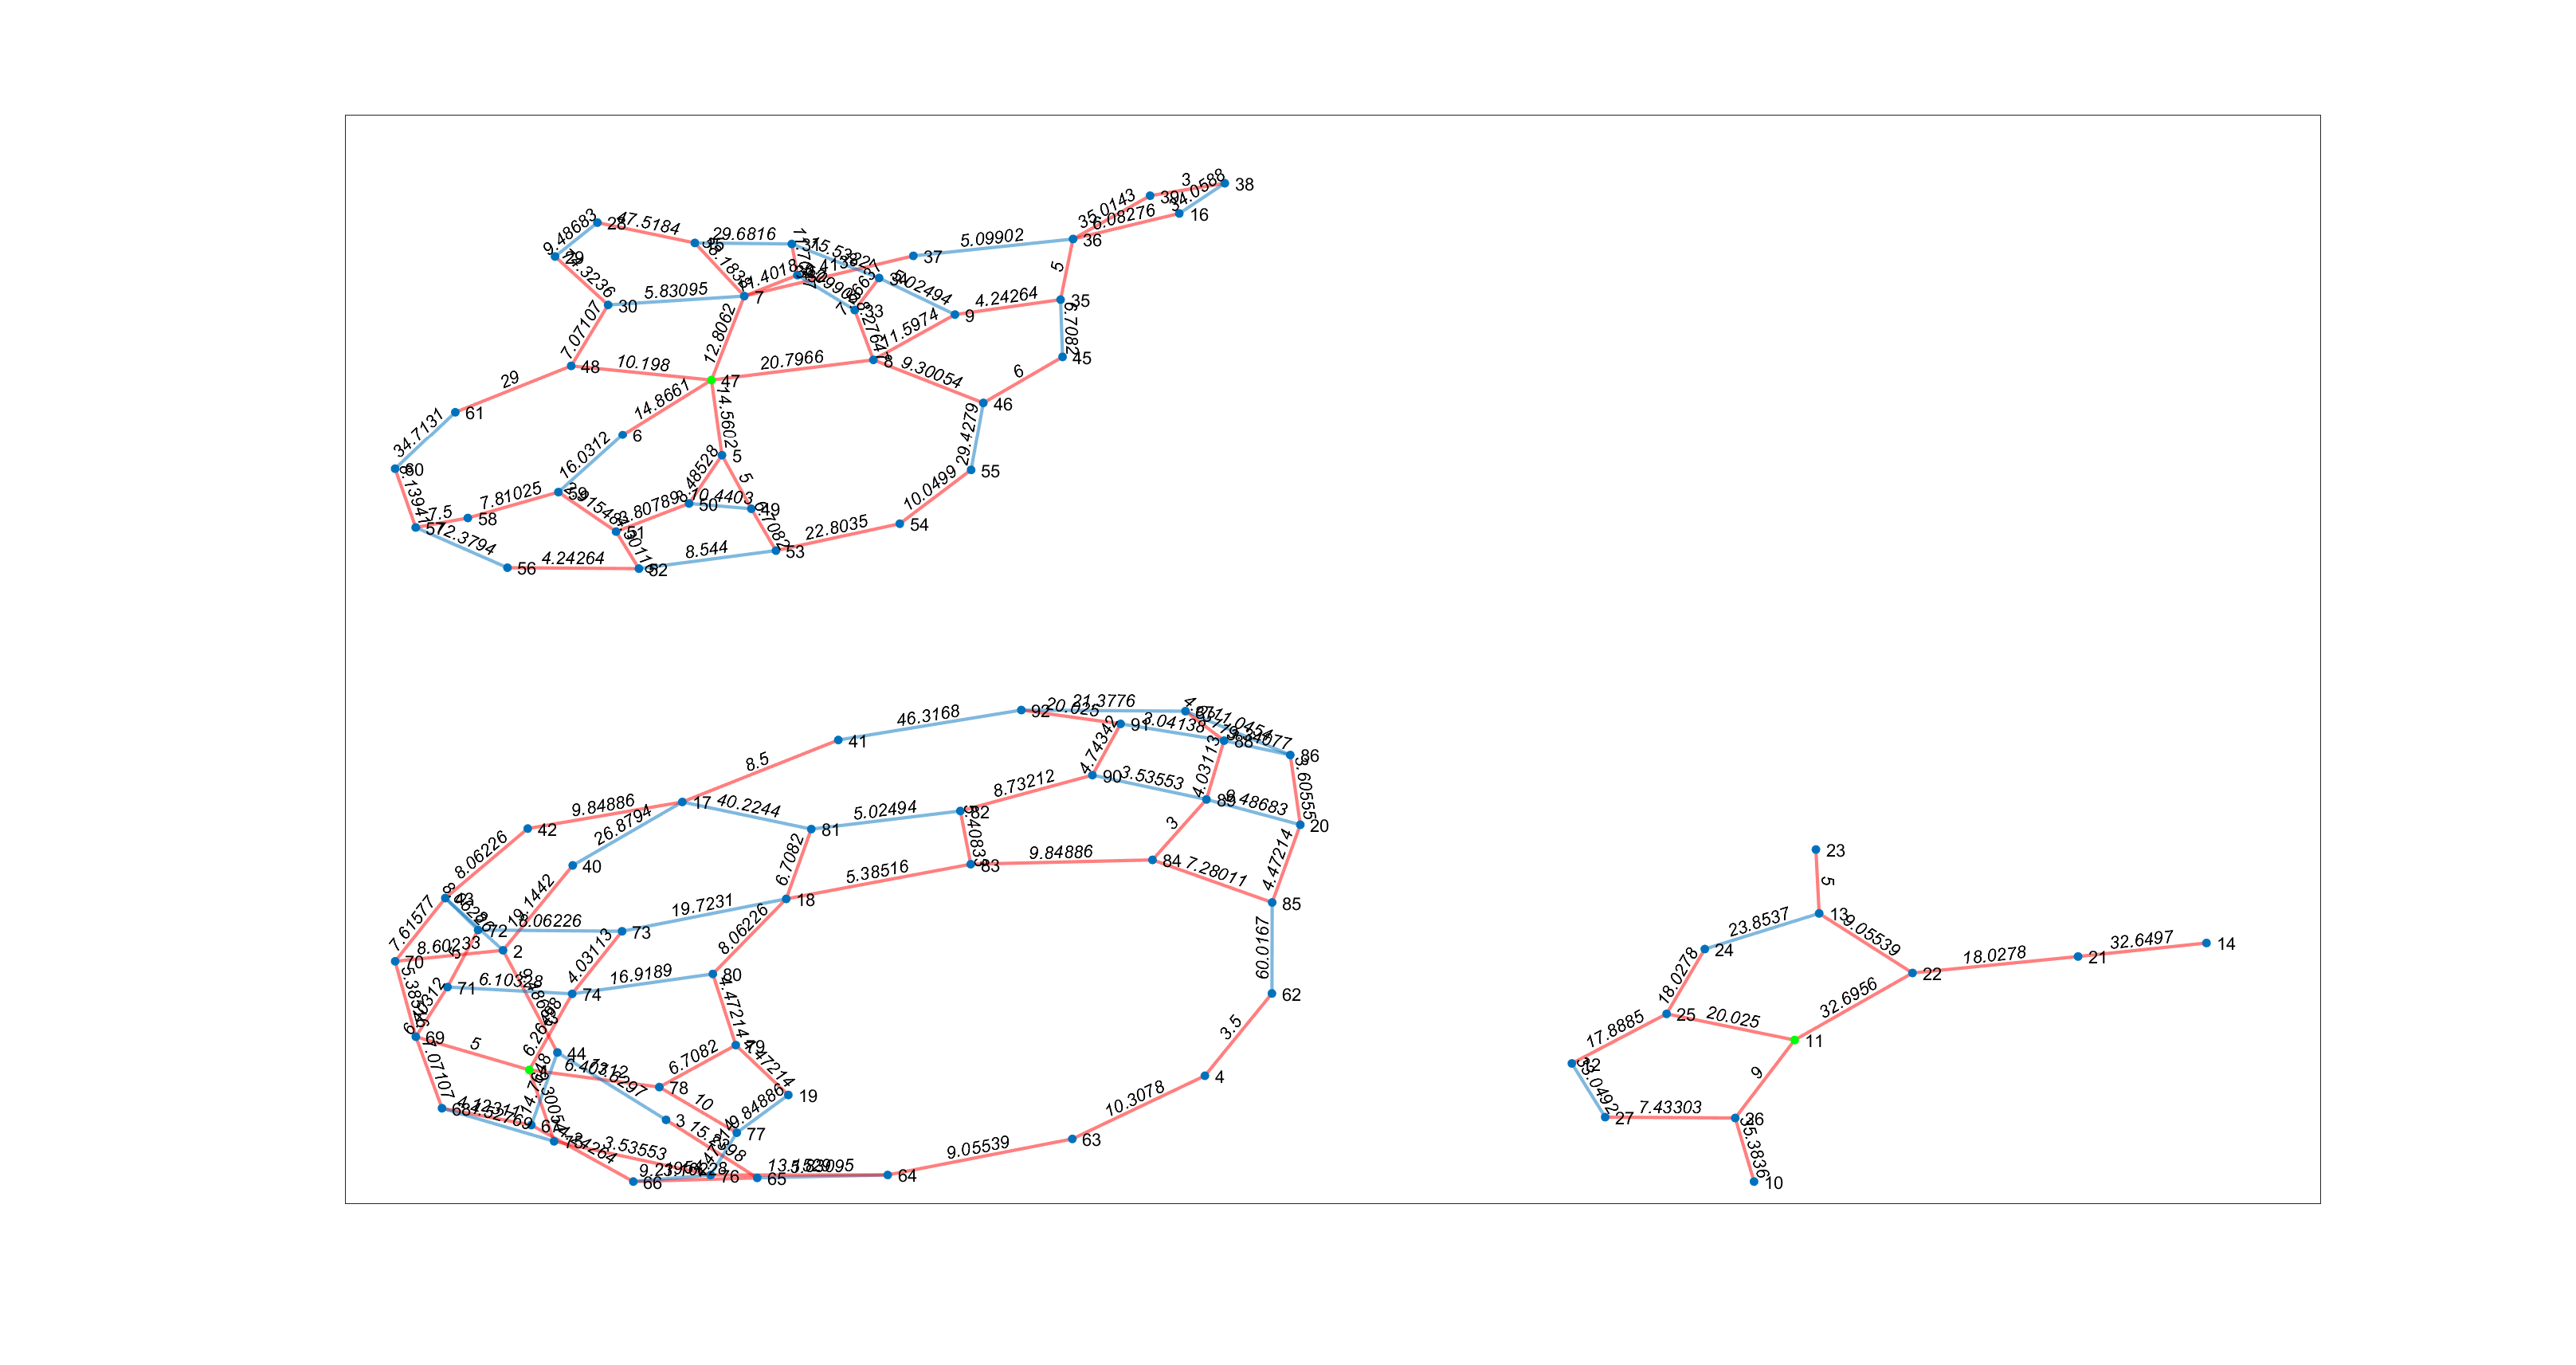
\includegraphics[height=10cm, width=16cm]{cluster3_red_G1.eps}
		\caption{赋权无向图}
		\label{fig:赋权无向图1}
	\end{figure}
	
	\subsubsection{求解最优配送站设置点}
	
	\textbf{Step1: 在每一簇中运用双层规划}
	
	在上层规划中,目标函数为:
	\begin{align*}
		{\rm{min}}~{F_u} = 0.5\sum\limits_{j \in J}^{} {{C_{j}}} {h_j} + 0.5\sum\limits_{i \in I}^{} {\sum\limits_{j \in J}^{} {{D_{ij}}} } {z_{ij}}
	\end{align*}
	
	约束条件为:
	\begin{align*}
			s.t.\left \{{\begin{matrix}\sum_{j\in J}^{}{{{z}_{ij}}}=1,&&i\in I&\\&&&\\{{z}_{ij}}≤h,&&i\in I&j\in J\\&&&\\\sum_{j\in J}^{}{{{h}_{j}}=K}&&&\\&&&\\{{z}_{ij}},{{h}_{j}}\in \{0,1\},&&i\in I&j\in J\end{matrix}}\right .
	\end{align*}
	
	在下层规划中,目标函数为:
	\begin{align*}
		{\rm{min }}{F_2} = \sum\limits_{j \in J}^{} {T{C_{nj}}} {h_j} + \sum\limits_{j \in J}^{} {n{C_n}} {h_j}
	\end{align*}
	
	约束条件:
	
	\begin{align*}
		s.t.\left \{{\begin{matrix}\sum_{i\in I}^{}{\sum_{n\in N}^{}{{{y}_{jin}}}}-{{h}_{j}}\le 0,&&i\in I&j\in J\\\sum_{n\in N}^{}{{{y}_{ijn}}}\le 1,&&i\in I&j\in J\\\sum_{n\in N}^{}{{{w}_{n}}}=N-1&&&\end{matrix}}\right.
	\end{align*}
	
	
	\textbf{Step2: 绘制出有3个配送中心时的最优配送站的设置方案}
	
	利用Matlab,求解得出最优配送站设置方案如图\ref{fig:最优配送站设置方案}所示:
	\begin{figure}[htbp]
		\centering
		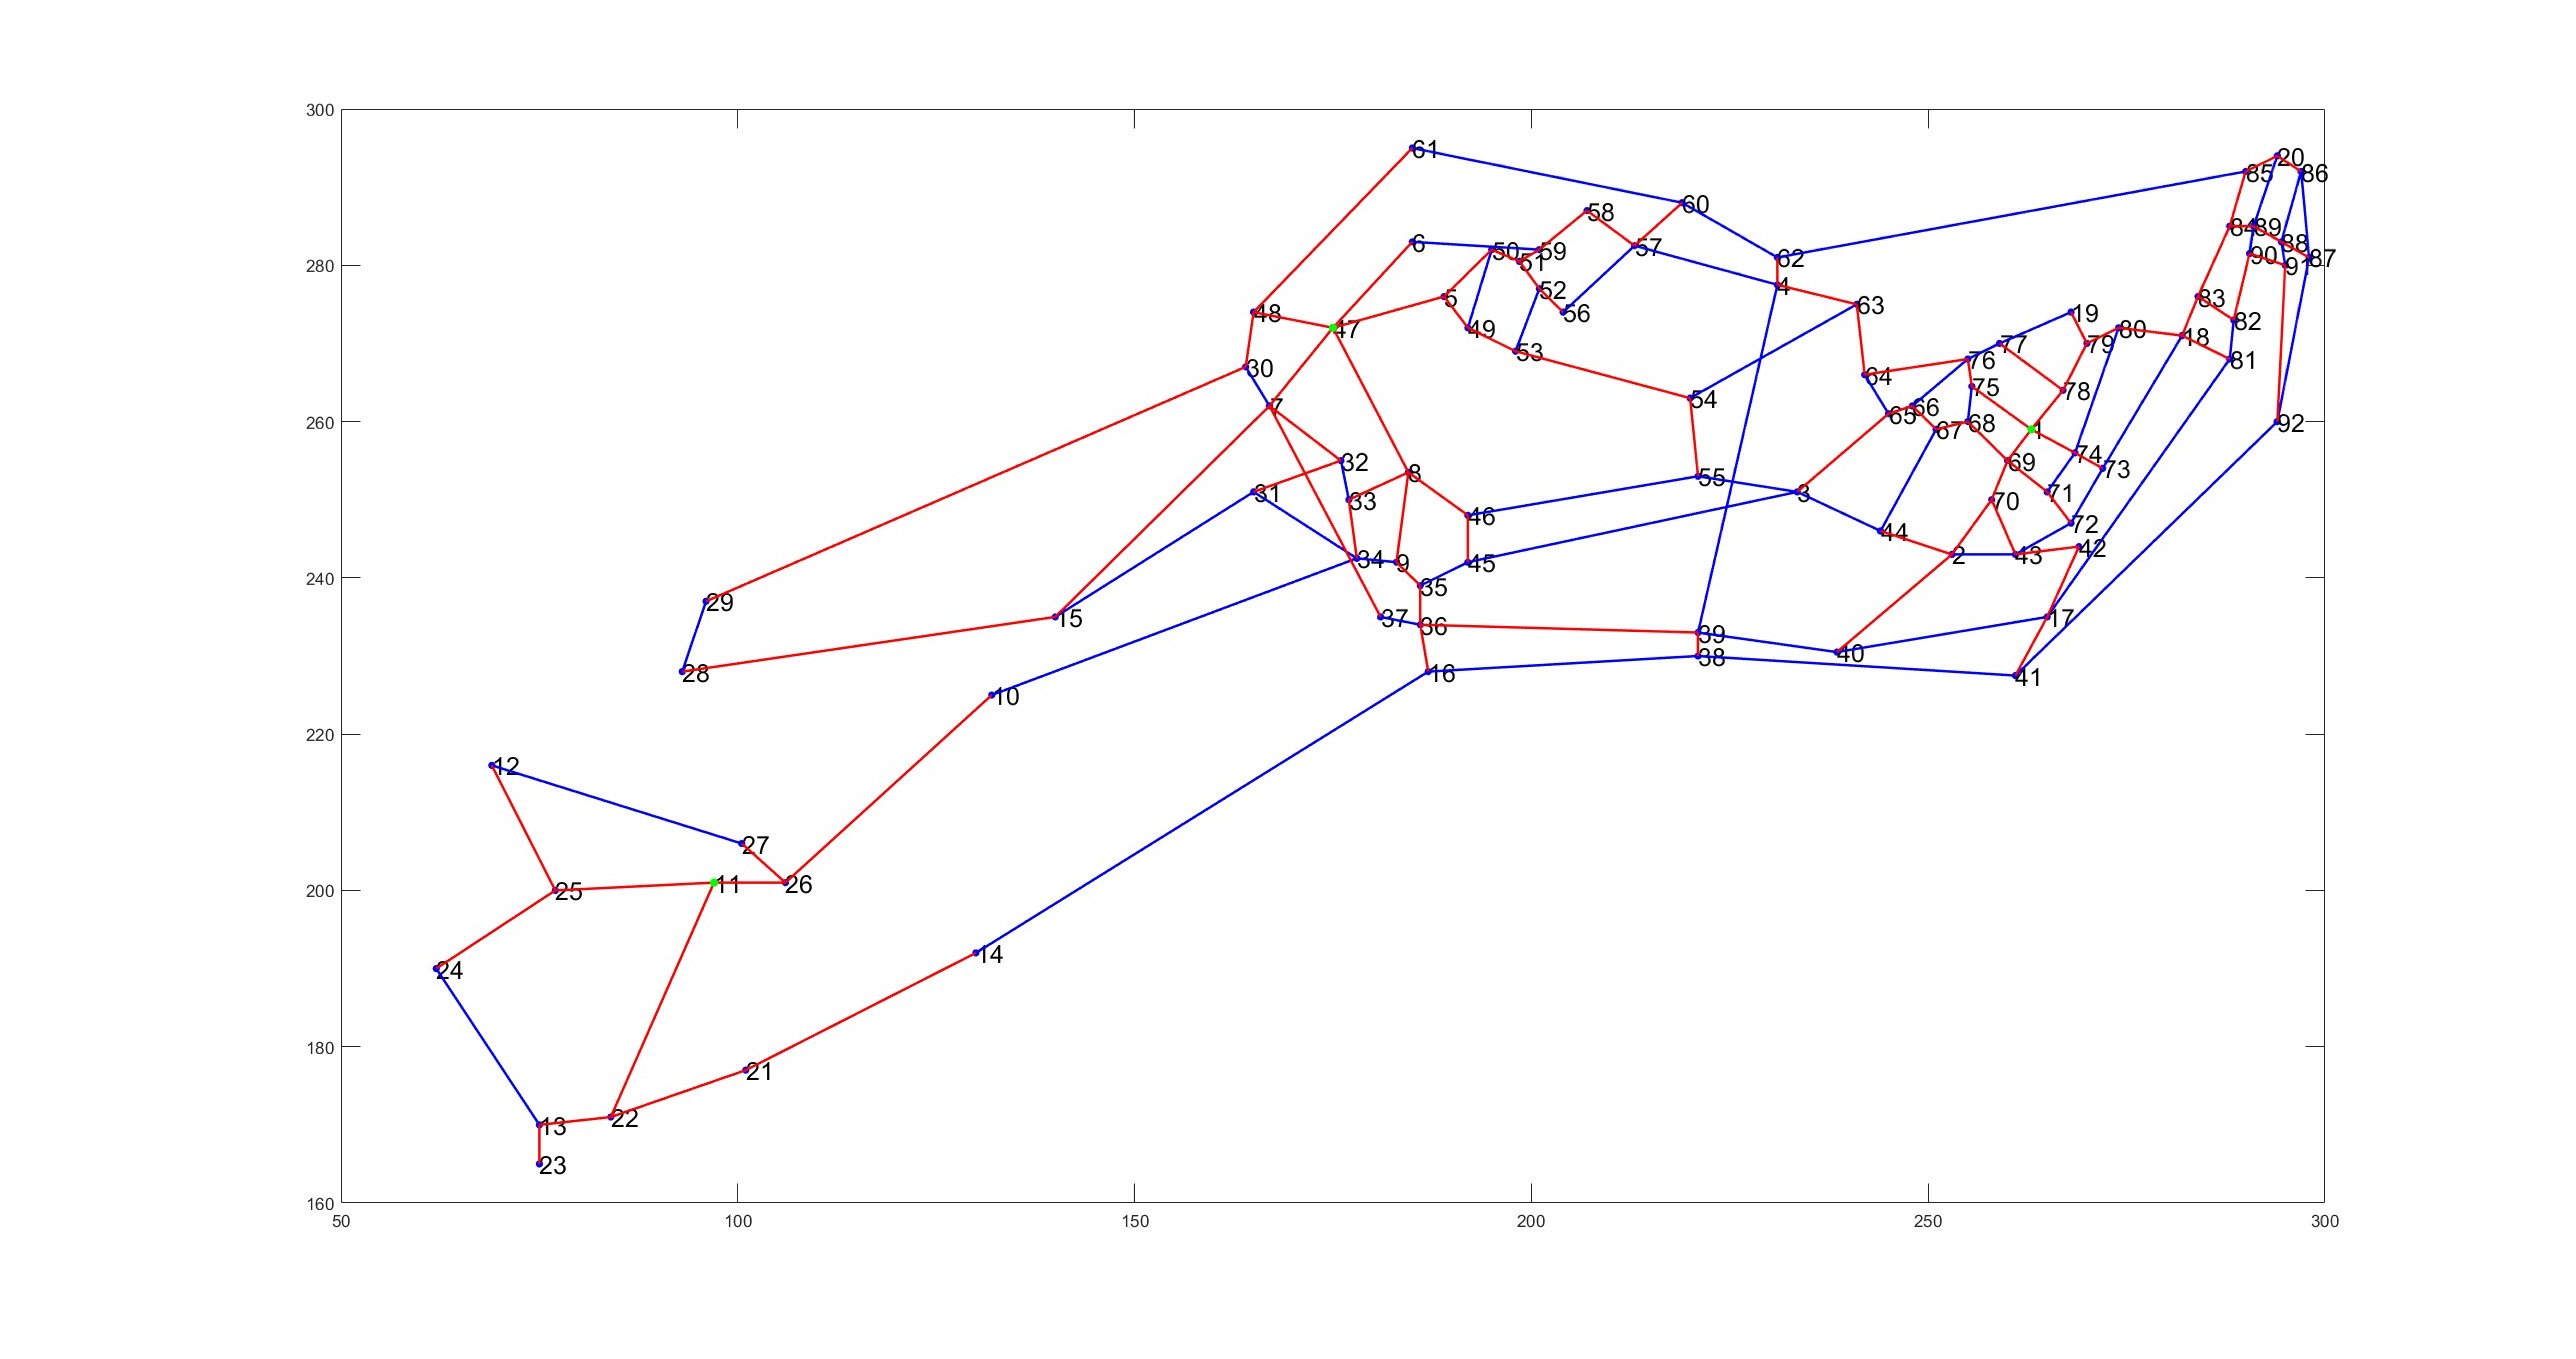
\includegraphics[width=16cm]{cluster3_real_red_G1.eps}
		\caption{最优配送站设置方案}
		\label{fig:最优配送站设置方案}
	\end{figure}
	
	图中的的蓝色节点为网点,绿色节点为配送站,蓝线为非运送路径,红线为运送路径。
	
	即设置1、47、11号网点为鲜奶配送站。同时由matlab可计算出此设置方案下的配送路径总长度$S_3$=3039.413 $m$
	
\textbf{Step3: 绘制出有1个配送中心时的最优配送站的设置方案进行对比}

同时,在不进行聚类的情况下,通过双层规划得出了仅设置一个配送站时的最佳设置网点(3号网点)与配送路径,如图\ref{fig:最佳设置网点(3号网点)与配送路径}所示:

	\begin{figure}[htbp]
		\centering
		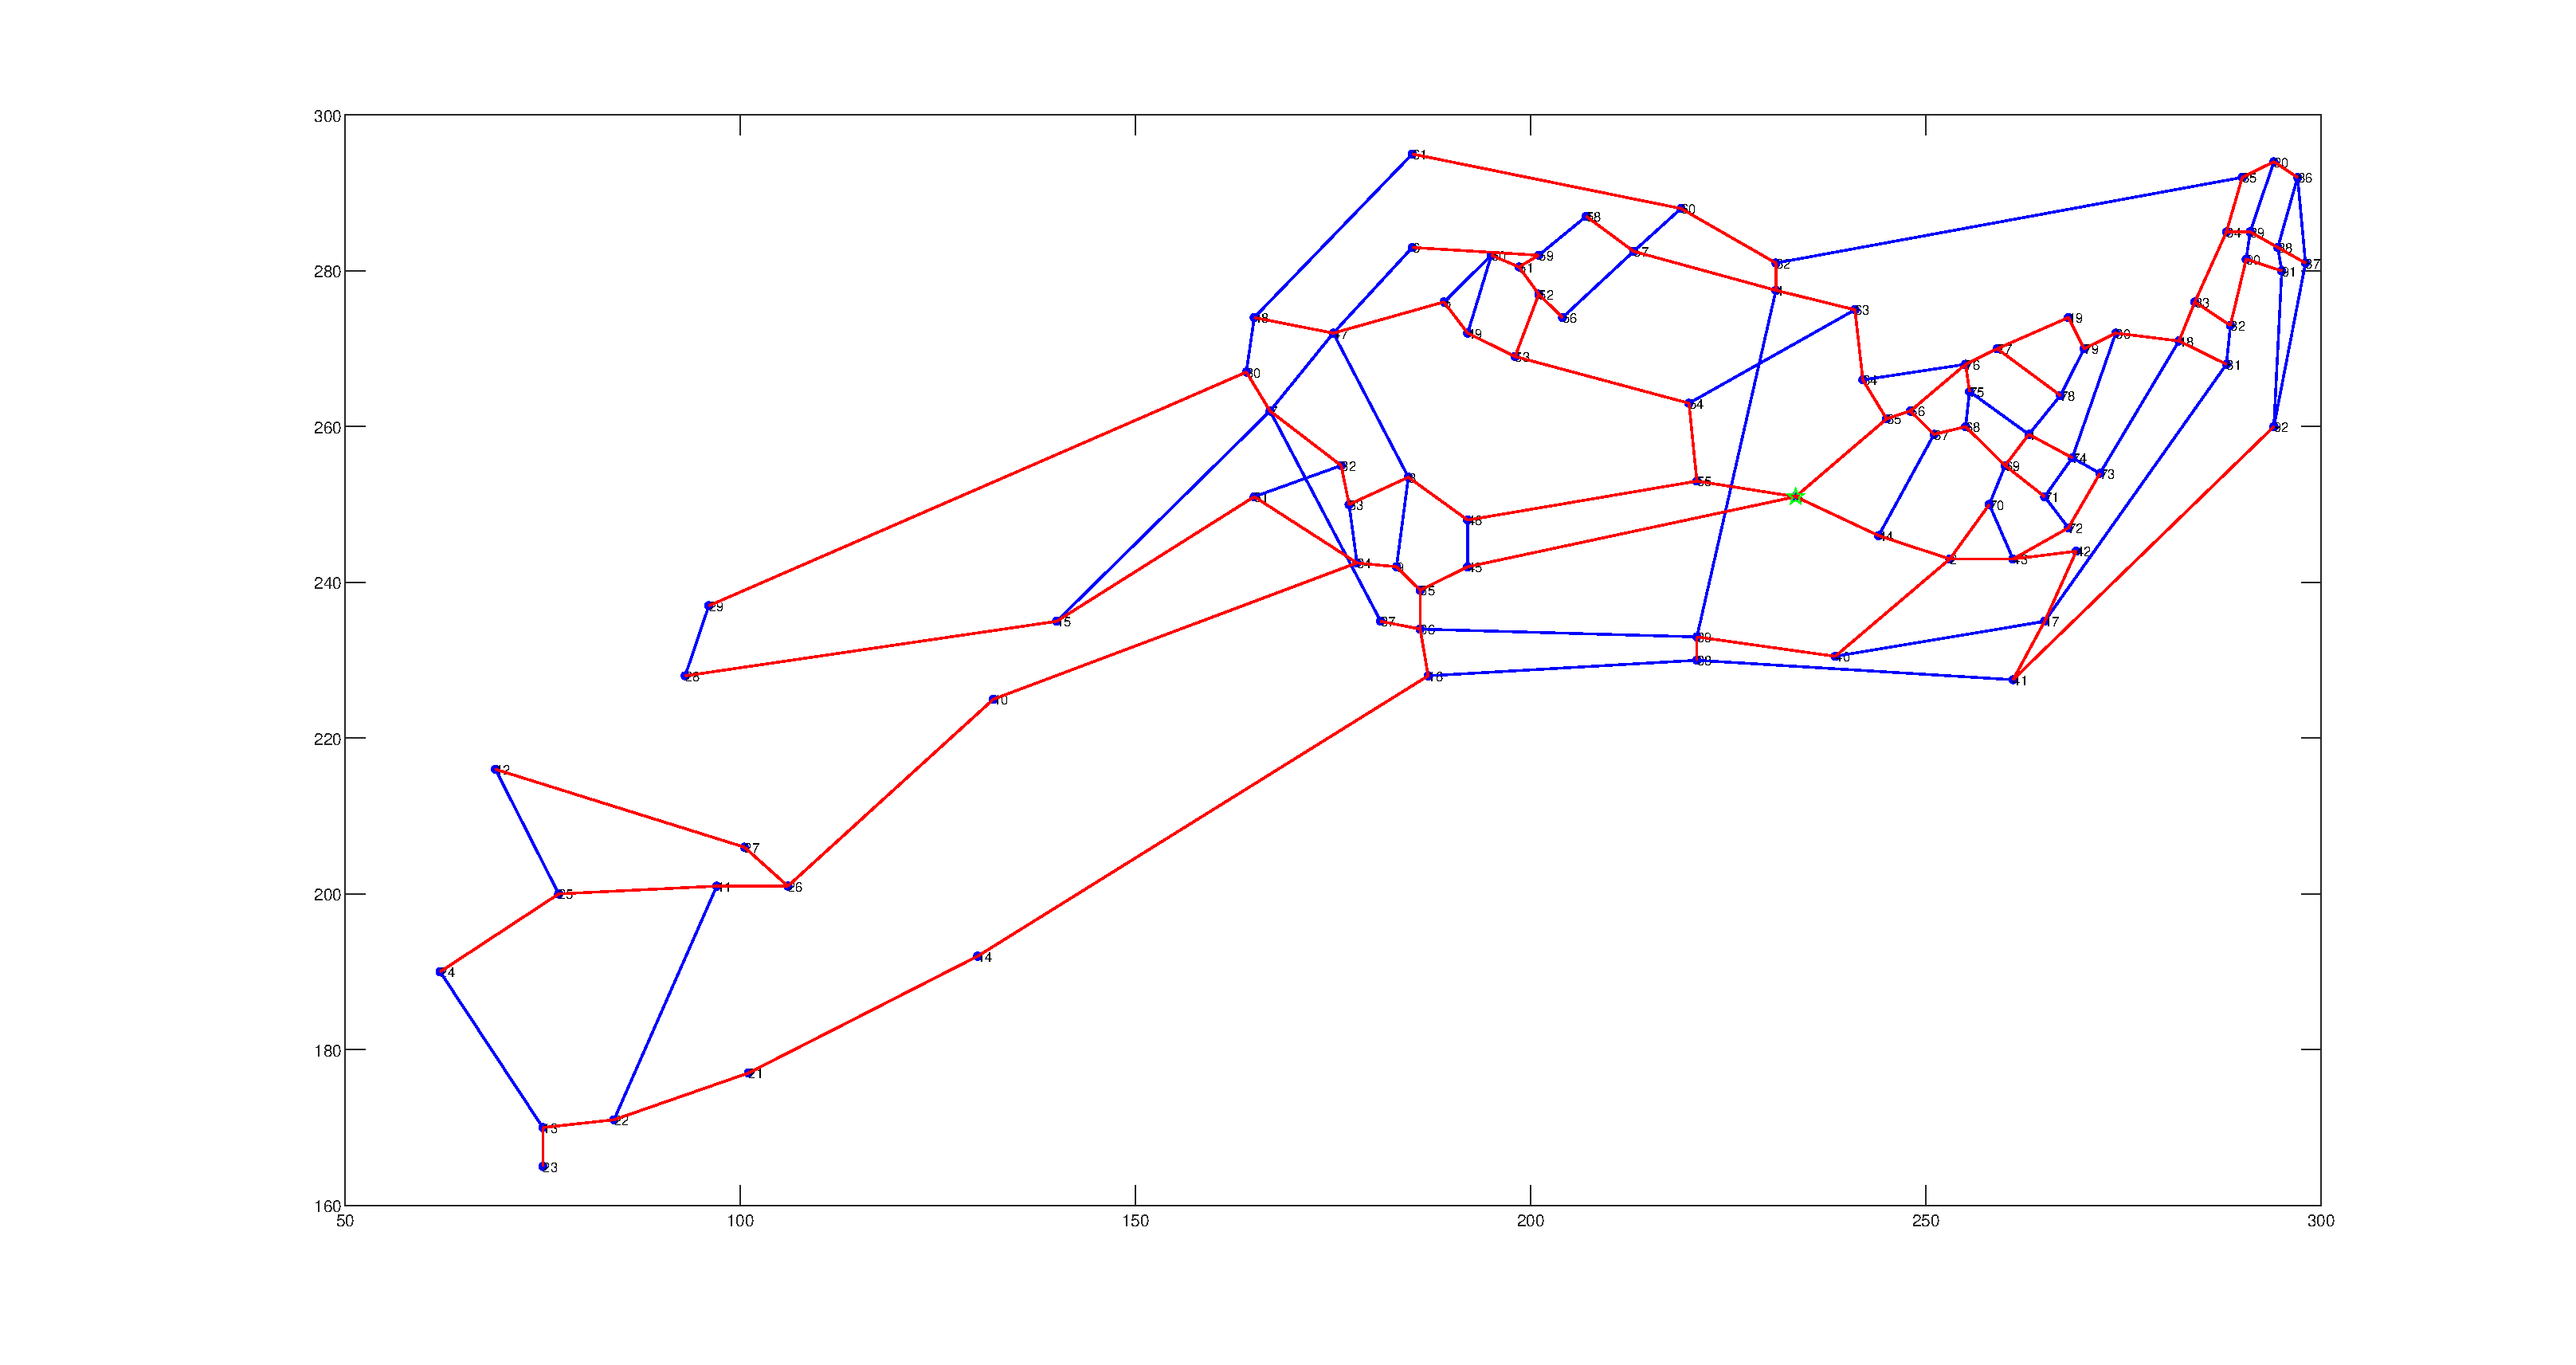
\includegraphics[ width=16cm]{real_red_G.eps}
		\caption{最佳设置网点(3号网点)与配送路径}
		\label{fig:最佳设置网点(3号网点)与配送路径}
	\end{figure}

%由两图的对比可见选取三个配送站点走的路径与只选取一个站点相比明显变少。
得到该设置方案下的配送路径总长度$S_1$=6393.765 $m$。

比较与易得:$S_1>S_3$,即在设置1、47、11三个网点作为鲜奶配送站,可以在尽量缩短配送在途时间的条件下,使配送站设置方案最经济。
	
	\subsection{求解结果}
问题一求解结果如下表所示:
	
	\begin{table}[h]
		\centering
		\caption{问题一求解结果}
		\begin{tabular}{ccccc} 
			\hline
			设定配送站个数 & 配送站网点号  & 总距离     & 需要物流车数量 & 总成本  \\ 
			\hline
			1       & 3       & 6393.77 & 24      & 较高   \\
			3       & 47,1,11 & 3039.41 & 32      & 较低   \\
			\hline
		\end{tabular}
	\end{table}


对比表中数据,由于本文模型假设每辆非冷链小型物流车的时速恒定不变,不受道路车流量影响,故尽量缩短配送总距离即可满足尽量缩短配送时间的题设条件,故而选择网点1、11、47三个网点设置配送站是在尽量缩短配送距离的条件下,总成本较低的最经济的鲜奶配送站设置方案。	
	%本文模型建立中,上层规划中,建设成本、鲜奶配送成本与最短配送距离的数量级差距较小,无需进行归一化处理;但量纲不同,应先进行无量纲处理,本文采用线性加权法(线性加权法关键是要确定每个目标的权重,它反映不同目标在决策者心中的重要程度,重要程度高的权重就大,重要程度低的权重就小。相较于ε约束法、理想点法等方法更为简便、快捷)。
	%本题对于成本与距离的期望权重均取0.5,则上层规划变换如下:
	\section{问题二的模型的建立和求解}
	\subsection{模型建立}

	\subsubsection{建立同问题一相同的数学模型}
本题要求配送站在10分钟内将鲜奶配送到网点,同时给出物流车的时速为$20km/h=\frac{1000}{3}m/min$,因而已知条件有物流车时速为$20km/h=\frac{1000}{3}m/min$,配送时间阈值为$t=10\min{}$,由运动学公式$s=\frac{v}{t}$可得二维坐标图中配送点的最大配送范围为$s=3333.33m$。此处需注意附录中规定坐标的单位长度为1毫米且给定比例尺为:图上距离:实际距离=$1mm:10m$ ,故按附录所给比例可得二维坐标图中的配送站的最大辐射距离为$d$=333.33 $m$。
	
	\subsubsection{在问题一所建立模型的基础上改进双层规划}
对于问题二,上层规划在第一问基础上,增加一个约束条件:${{D}_{ij}} \le d$ ,表示网点在配送站的配送范围内,$d$表示新建配送站配送距离上限。

\textbf{Step1: 建立上层规划模型}

\textbf{上层规划模型:}用于确定配送中心最优选址。题述中,鲜奶配送站应做到在配送在途时间尽可能短的同时最经济地配送鲜奶。

据此可以得到目标函数应由鲜奶配送站的总建设成本、配送点与各网点间的距离之和,以及鲜奶配送成本三者之和组成,并且应取其最小值,则目标函数为:
	
		\begin{align*}
		{\rm{min}}~{{F}_{u}}=\sum_{j\in J}^{}{{{C}_{j}}}{{h}_{j}}+\sum_{i\in I}^{}{\sum_{j\in J}^{}{{{D}_{ij}}}}{{z}_{ij}}
	\end{align*}
此目标函数中,建设成本与最短配送距离的数量级差距较小,无需进行归一化处理;但两者的量纲不同,应用线性加权法进行无量纲处理。由于本问中题干限制配送距离,要求考虑建设成本,故本问对于成本与距离两个子目标的期望权重分别取0.8与0.2,则上层规划的目标函数变换如下:
	\begin{align*}
	{\rm{min}}~min{{F}_{u}}=0.8\sum_{j\in J}^{}{{{C}_{j}}}{{h}_{j}}+0.2\sum_{i\in I}^{}{\sum_{j\in J}^{}{{{D}_{ij}}}}{{z}_{ij}}
	\end{align*}
	目标函数的约束条件为:
	\begin{align*}
		s.t.\left \{{\begin{matrix}\sum_{j\in J}^{}{{{z}_{ij}}}=1,&&i\in I&\\&&&\\{{z}_{ij}}\le h,&&i\in I&j\in J\\&&&\\\sum_{j\in J}^{}{{{h}_{j}}=K}&&&\\&&&\\{{D}_{ij}}\le d,&&i\in I&j\in J\\&&&\\{{z}_{ij}},{{h}_{j}}\in \{0,1\},&&i\in I&j\in J\end{matrix}}\right .
	\end{align*}


\textbf{Step2: 建立下层规划模型}

\textbf{下层规划模型}:用于确定鲜奶最佳配送路径,即行驶最短行程、使用最少时间、花费最低成本完成鲜奶配送任务。题述鲜奶配送站的任务就是在缩短配送在途时间,限制配送鲜奶配送站配送范围的条件下,最经济地配送鲜奶。目标函数是由鲜奶配送站的总建设成本、配送点与各网点间的距离两者之和最小,目标函数公式表达如下:
	\begin{align*}
		{\rm{min}}~{{F}_{2}}=\sum_{j\in j}^{}{T{{C}_{nj}}}{{h}_{j}}+\sum_{j\in j}^{}{n{{C}_{n}}}{{h}_{j}}+\sum_{j\in j}^{}{{{C}_{j}}}{{h}_{j}}
	\end{align*}

其约束条件为:
	\begin{align*}
s.t.\left \{{\begin{matrix}\sum_{i\in I}^{}{\sum_{n\in N}^{}{{{y}_{jin}}}}-{{h}_{j}}\le 0,&&i\in I&j\in J\\&&&\\\sum_{n\in N}^{}{{{y}_{ijn}}}\le 1,&&i\in I&j\in J\\&&&\\\sum_{n\in N}^{}{{{w}_{n}}}=N-1&&&\\&&&\end{matrix}}\right .
	\end{align*}
	

	
	
	\subsection{模型求解}
对于问题一所选择配送站配送方案判中,设每一个鲜奶配送点的最大配送距离,通过比较与d(二维坐标图中配送点的最大配送距离)两者的大小,判断问题一中的配送站设置方案是否符合问题二所要求的配送辐射范围。

利用Matlab,可得出${{M}_{1}}=69.93<d$,${{M}_{11}}=83.37<d$,${{M}_{47}}=72.72<d$
	故问题一所得鲜奶配送站的设置方案依旧符合问题二的题设条件。
	
	\subsection{求解结果}
% \usepackage{multirow}
% \usepackage{multirow}
问题二求解结果如下表所示:

\begin{table}[h]
	\centering
	\caption{问题二求解结果}
	\begin{tabular}{cccc} 
		\hline
		配送站网点号 & 最远单配送路径 & 配送范围阈值                  & 是否符合题设要求  \\ 
		\hline
		47     & 72.73   & \multirow{3}{*}{333.33} & 符合        \\
		1      & 83.37   &                         & 符合        \\
		11     & 69.93   &                         & 符合        \\
		\hline
	\end{tabular}
\end{table}

对图表数据分析可知,问题一所得鲜奶配送站的设置方案依旧符合问题二对鲜奶配送站最远配送距离的限制。即最优的配送站点设置方案为:设置网点1、11、47为鲜奶配送站点。

\section{问题三的模型的建立与求解}
\subsection{模型建立}	
对于问题三,需在问题二所建双层规划模型基础上额外考虑配送量对建站点的影响,改进双层规划流程图如下:
	\begin{figure}[htbp]
	\centering
	\includegraphics[width=0.4\linewidth]{framework2.pdf}
	\caption{问题三双层规划流程图}
	\label{fig:双层规划流程图2}
\end{figure}	

\textbf{Step1: 建立上层规划模型}

\textbf{上层规划模型:}用于确定配送中心最优选址。题述鲜奶配送站的任务就是在缩短配送在途时间,限制配送鲜奶配送站配送范围的条件下,最经济地配送鲜奶。

目标函数是鲜奶配送站的总建设成本、配送点与各网点间的距离两者之和最小,目标函数表达式为:
	
\begin{align*}
	min{{F}_{u}}=\sum_{j\in J}^{}{{{C}_{j}}}{{h}_{j}}+\sum_{i\in I}^{}{\sum_{j\in J}^{}{{{D}_{ij}}}}{{z}_{ij}}
\end{align*}	


	
	由于此目标函数中,建设成本与最短配送距离的数量级差距较小,无需进行归一化处理;但两者的量纲不同,应用线性加权法进行无量纲处理。由于本问中要求配送量均衡,从而避免造成资源浪费或延误配送,而建设成本的要求较松散,故本问对于成本与距离两个子目标的期望权重分别取0.3与0.7,则上层规划的目标函数变换如下:
	
\begin{align*}
	min{{F}_{u}}=0.3\sum_{j\in J}^{}{{{C}_{j}}}{{h}_{j}}+0.7\sum_{i\in I}^{}{\sum_{j\in J}^{}{{{D}_{ij}}}}{{z}_{ij}}
\end{align*}
	
	其约束条件为:
	
\begin{align*}
	s.t.\left \{{\begin{matrix}\sum_{j\in J}^{}{{{z}_{ij}}}=1,&&i\in I&\\&&&\\{{z}_{ij}}\le h,&&i\in I&j\in J\\&&&\\\sum_{j\in J}^{}{{{h}_{j}}=K}&&&\\&&&\\{{D}_{ij}}\le d,&&i\in I&j\in J\\&&&\\{{z}_{ij}},{{h}_{j}}\in \{0,1\},&&i\in I&j\in J\end{matrix}}\right .
\end{align*}
	
\textbf{Step2: 建立下层规划模型}
	
\textbf{下层规划模型:}用于确定鲜奶最佳配送路径,即行驶最短行程、使用最少时间、花费最低成本完成鲜奶配送任务。

据此可以得到目标函数应由车辆的配送成本和车辆的固定使用成本之和组成,并且应取其最小值,三者量纲相同,数量级差距较小,无需对目标函数进行无量纲化处理,则目标函数为:

\begin{align*}
	min{{F}_{2}}=\sum_{j\in J}^{}{T{{C}_{nj}}}{{h}_{j}}+\sum_{j\in J}^{}{n{{C}_{n}}}{{h}_{j}}+\sum_{i\in I}^{}{\sum_{j\in J}^{}{{\omega _{i}}}}{{r}_{ij}}{{D}_{ij}}
\end{align*}
	
	式中,$\sum_{i\in I}^{}{\sum_{j\in J}^{}{{{ω}_{i}}}}{{r}_{ij}}{{D}_{ij}}$表示鲜奶配送成本。${{r}_{ij}}$表示网点$i$与配送站$j$之间配送鲜奶的单位成本,${{\omega }_{i}}$表示网点i的订奶量。
	
	其约束条件为:
	
	\begin{align*}
		s.t.\left \{{\begin{matrix}\sum_{i\in I}^{}{\sum_{n\in N}^{}{{{y}_{jin}}}}-{{h}_{j}}\le 0,&&i\in I&j\in J\\\sum_{n\in N}^{}{{{y}_{ijn}}}\le 1,&&i\in I&j\in J\\\sum_{n\in N}^{}{{{w}_{n}}}=N-1&&&\end{matrix}}\right.
	\end{align*}
	
\subsection{模型求解}	

\subsubsection{依据问题一二聚类结果进行均衡鲜奶配送量的修订}

若要均衡配送站的配送量,需要对网点进行新的规划,从而保证每一配送站点的配送量在均衡区间$\left [{0.9\bar{x},1.1\bar{x}}\right ]$内,目标函数表达式为:
\begin{align*}
	0.9\bar{x}\le {{p}_{h}}\le 1.1\bar{x}
\end{align*}

其中$h$表示第$h$个配站点,且$h\in \{1,2,...,K\}$,$K$为最优聚类数。

定义${{I}_{k}}$为聚类后每一簇的网点集合,即${{I}_{k}}=\{1,2,3,...,f\}$,${{ω}_{i}}$表示网点$i$的订奶量。

目标函数的约束条件为:

\begin{align*}
		s.t.\left \{{\begin{matrix}\bar{x}=\frac{1}{K}\sum_{i=1}^{92}{{{\omega }_{i}},}\\\\h\in \{1,2,...,K\},\\\\K=3,\\\\{{p}_{h}}=\sum_{k=1}^{K}{\sum\limits_{i\in {{I}_{k}}}{{{\omega }_{i}}}}\\\\\sum_{k=1}^{K}{{{I}_{k}}=92,}\end{matrix}}\right .
\end{align*}

网点重新分区规划后,单独由每一簇包含的所有网点对组$x,y$和权重向量$D$构建出三个赋权无向图如下:

\begin{figure}[htbp]
	\centering
	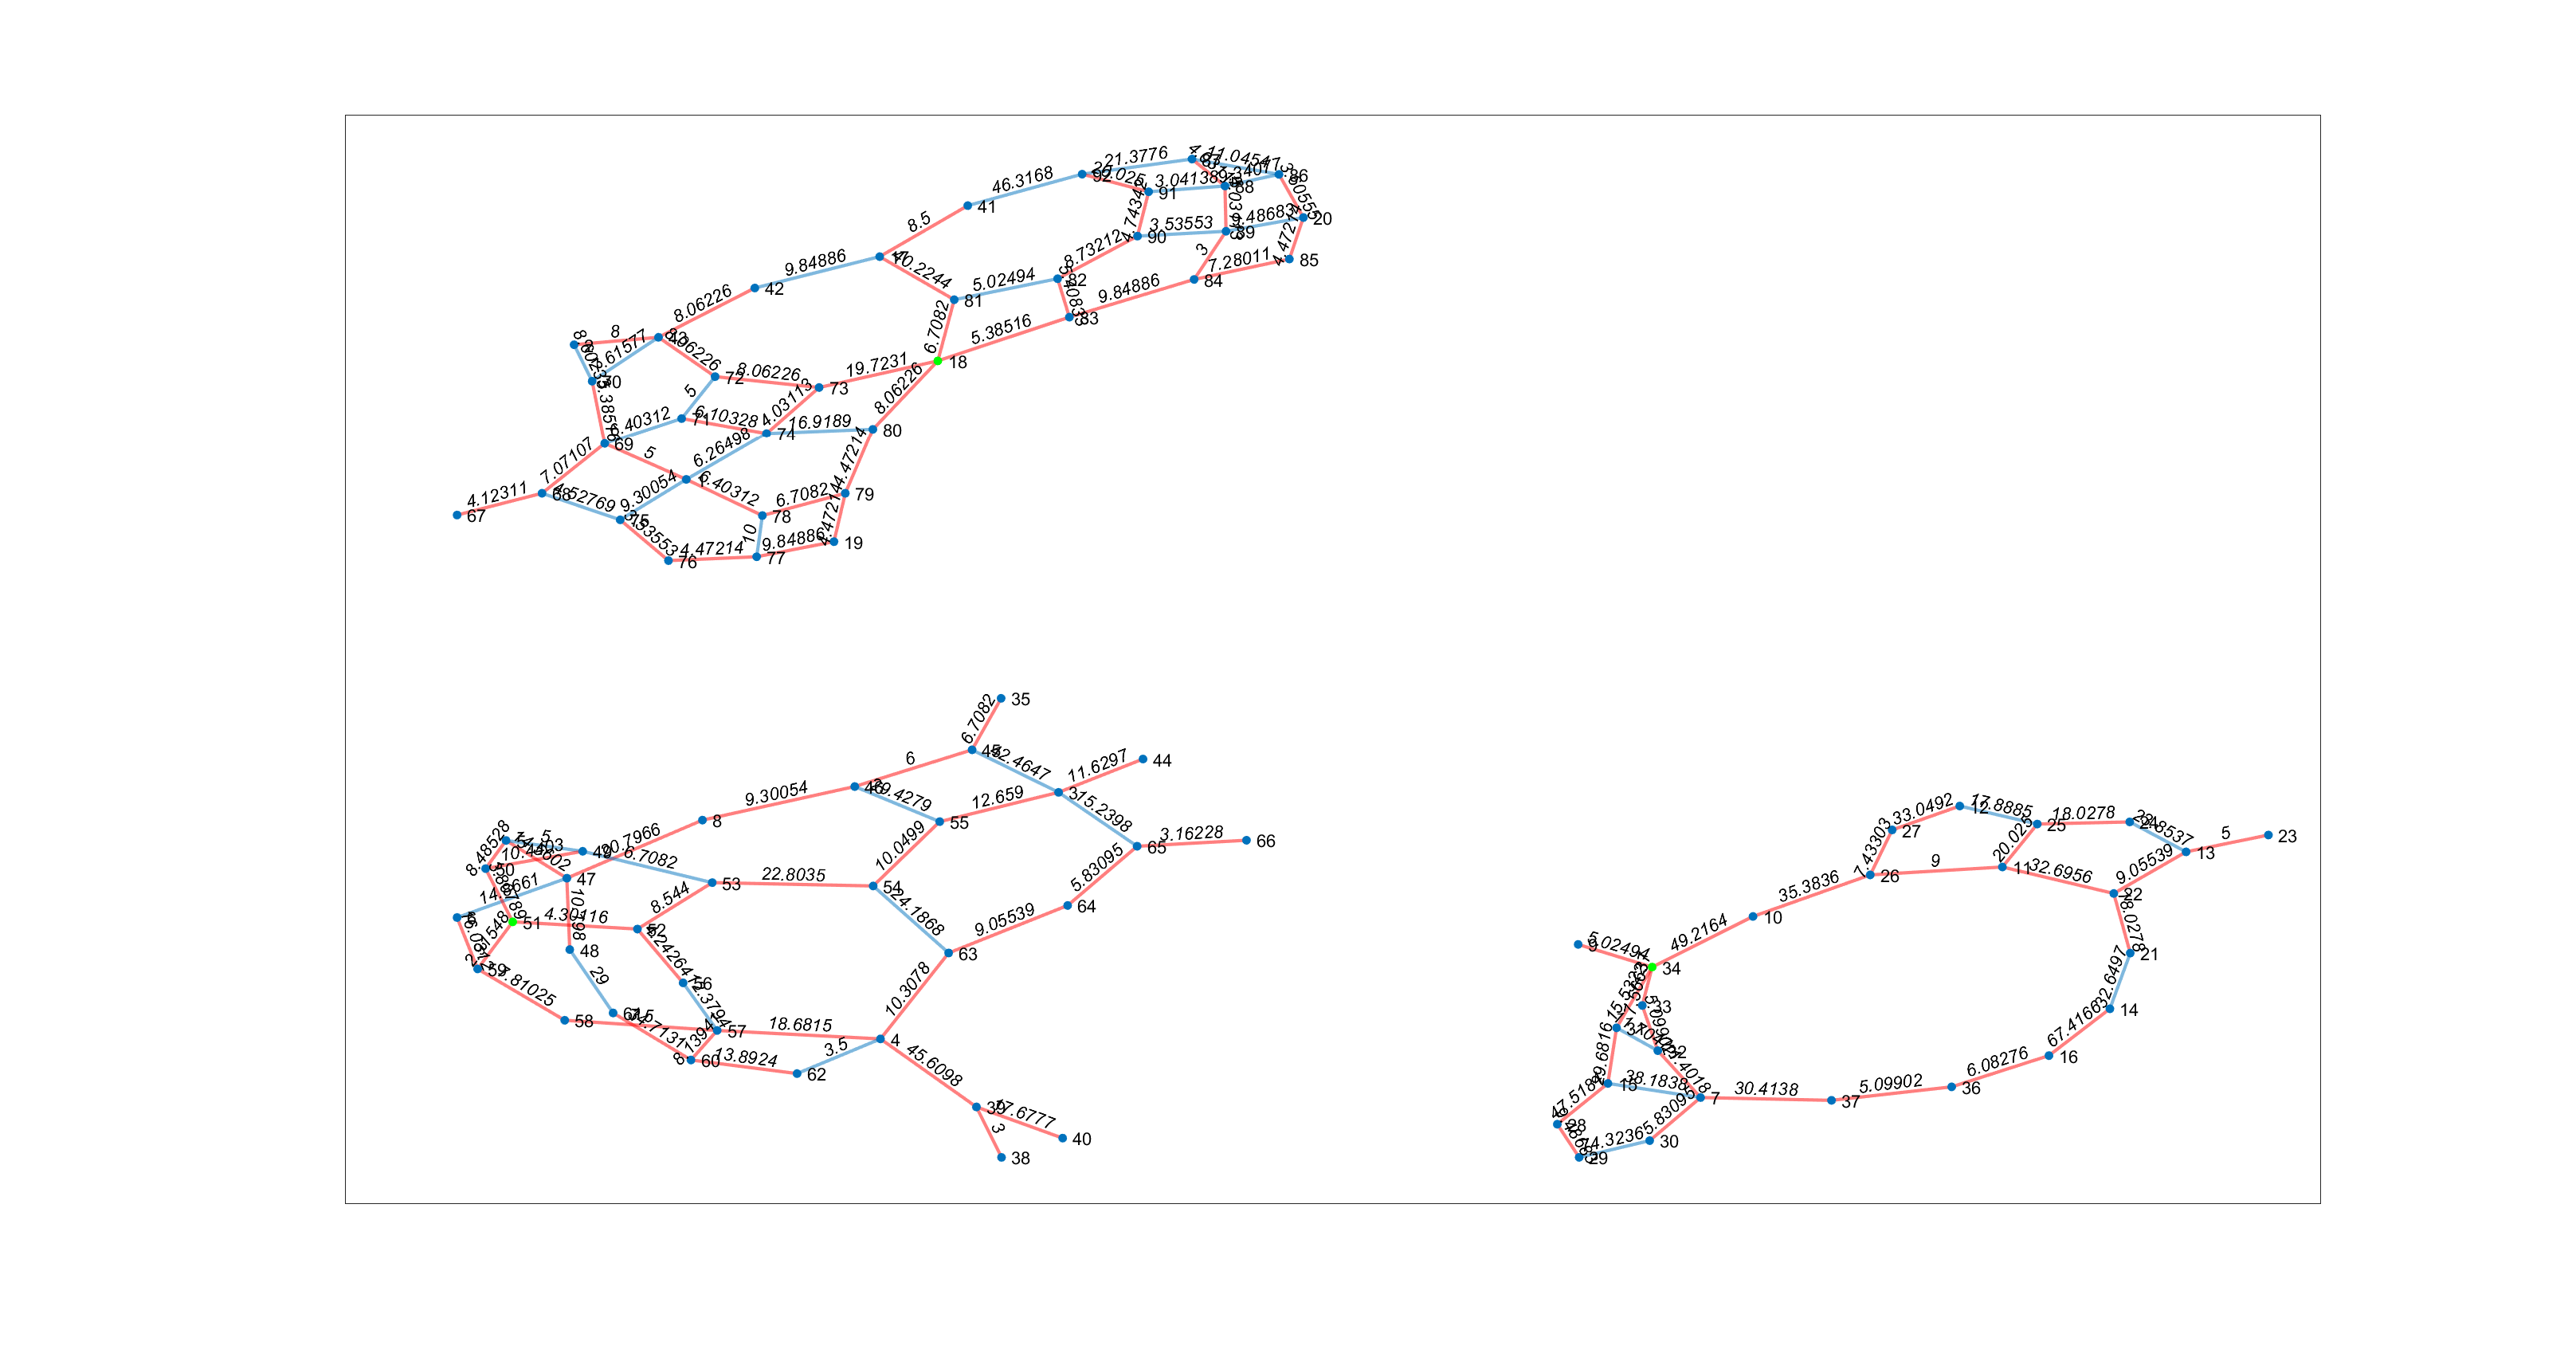
\includegraphics[width=0.85\linewidth]{figures/supply_G_red}
	\caption{均衡配送量后的的赋权无向图}
	\label{fig:supplygred}
\end{figure}




 \subsubsection{运用双层规划求解最优配送站的设置点}
上层规划的目标函数是鲜奶配送站的总建设成本、配送点与各网点间的距离两者之和最小,目标函数的表达式为:
\begin{align*}
	min{{F}_{u}}=0.3\sum_{j\in J}^{}{{{C}_{j}}}{{h}_{j}}+0.7\sum_{i\in I}^{}{\sum_{j\in J}^{}{{{D}_{ij}}}}{{z}_{ij}}
\end{align*}

其约束条件为:

\begin{align*}
	s.t.\left \{{\begin{matrix}\sum_{j\in J}^{}{{{z}_{ij}}}=1,&&i\in I&\\&&&\\{{z}_{ij}}\le h,&&i\in I&j\in J\\&&&\\\sum_{j\in J}^{}{{{h}_{j}}=K}&&&\\&&&\\{{D}_{ij}}\le d,&&i\in I&j\in J\\&&&\\{{z}_{ij}},{{h}_{j}}\in \{0,1\},&&i\in I&j\in J\end{matrix}}\right .
\end{align*}

下层规划的目标函数是车辆的配送成本、车辆的固定使用成本与鲜奶配送成本三者之和的最小值,目标函数表达式为:

\begin{align*}
	min{{F}_{2}}=\sum_{j\in J}^{}{T{{C}_{nj}}}{{h}_{j}}+\sum_{j\in J}^{}{n{{C}_{n}}}{{h}_{j}}+\sum_{i\in I}^{}{\sum_{j\in J}^{}{{\omega_{i}}}}{{r}_{ij}}{{D}_{ij}}
\end{align*}

式中,$\sum_{i\in I}^{}{\sum_{j\in J}^{}{{{ω}_{i}}}}{{r}_{ij}}{{D}_{ij}}$表示鲜奶配送成本。${{r}_{ij}}$表示网点$i$与配送站$j$之间配送鲜奶的单位成本,$\omega_{i}$表示网点i的订奶量。

其约束条件为:

\begin{align*}
s.t.\left \{{\begin{matrix}\sum_{i\in I}^{}{\sum_{n\in N}^{}{{{y}_{jin}}}}-{{h}_{j}}\le 0,&&i\in I&j\in J\\&&&\\\sum_{n\in N}^{}{{{y}_{ijn}}}\le 1,&&i\in I&j\in J\\&&&\\\sum_{n\in N}^{}{{{w}_{n}}}=N-1&&&\\&&&\end{matrix}}\right .
\end{align*}

利用Matlab求解,得到$J$=51、18、34。可绘制出最优配送站设置方案如图\ref{fig:supplyrealg1red}所示:

\begin{figure}[H]
	\centering
	\includegraphics[width=0.85\linewidth]{figures/supply_real_G1_red}
	\caption{最优配送站设置方案}
	\label{fig:supplyrealg1red}
\end{figure}

此时设立51号网点为配送点的总配送量$p_1$=3980,设立18号网点为配送点的总配送量$p_2$=4210,
设立34号网点为配送点的配送量$p_3$=4260。

\subsection{求解结果}
% \usepackage{multirow}
问题三求解结果如下表所示:

\begin{table}[h]
	\centering
	\caption{问题三求解结果}
	\begin{tabular}{cccc} 
		\hline
		配送站网点号 & 配送量  & 均衡区间                           & 配送量是否均衡  \\ 
		\hline
		51     & 3980 & \multirow{3}{*}{{[}3735,4565]} & 均衡       \\
		18     & 4210 &                                & 均衡       \\
		34     & 4260 &                                & 均衡       \\
		\hline
	\end{tabular}
\end{table}

对表中数据分析可知,在均衡各配送站的配送量的条件下,重新规划网点18、34、54为鲜奶配送站的设置方案,可以既不造成资源浪费,又不延误配送。





\section{模型评价}

\subsection{模型的优点}
\begin{itemize}
	\item 二维坐标图:二维坐标图直观易懂,能够有效地可视化数据,帮助人们更好地理解数据之间的关系和规律。 
	\item K-means聚类:是一种简单而有效的聚类算法,易于实现且计算速度快,适用于大规模数据集。数据点划分为K个簇,具有直观性和可解释性。
	\item 双层规划模型:能够在含有多个决策者或多个层次的决策问题中进行优化,在复杂系统中具有较好的适用性和解释性,可优化性高。
\end{itemize}


\subsection{模型的缺点}
\begin{itemize}
	\item 二维坐标图:在高维数据集上失去了效果,无法很好地展示多维数据的复杂性和关联性。
	\item K-means聚类:K-means对初始质心的选择敏感,可能收敛于局部最小值。此外,K-means假设簇的形状是球形的(本文对二维坐标系的网点进行聚类,簇的形状是圆形),对非球形簇效果不佳,会导致聚为一类的网点间并无直接或间接的道路连接。
	\item 双层规划:复杂度较高,计算成本大,求解过程可能非常耗时。此外,在本文实际的应用过程中,参数的设定和问题的建模较难,需考虑因素较为复杂。
\end{itemize}
	%\subsection{模型的推广}
	
	%参考文献
	%	\begin{thebibliography}{9}%宽度9
		%		\bibitem[1]{liuhaiyang2013latex}
		%		刘海洋.
		%		\newblock \LaTeX {}入门\allowbreak[J].
		%		\newblock 电子工业出版社, 北京, 2013.
		%		\bibitem[2]{mathematical-modeling}
		%		全国大学生数学建模竞赛论文格式规范 (2020 年 8 月 25 日修改).
		%		\bibitem{3} \url{https://www.latexstudio.net}
		%	\end{thebibliography}
	
	%\section{参考文献}
	\newpage
	
	\nocite{*}
	%\addcontentsline{toc}{section}{参考文献}
	%\bibliographystyle{bib/gbt7714-2005}
	
	\bibliographystyle{gbt7714-numerical}
	%\bibliographystyle{unsrt}
	%\bibliographystyle{IEEEtran}
	\bibliography{bib/ref.bib}
	
	\newpage
	%附录
	
    \begin{appendices}
    	
	\section{代码文件列表}
	% Table generated by Excel2LaTeX from sheet 'Sheet1'
	\begin{table}[htbp]
		\centering
		\caption{Add caption}
		\begin{tabularx}{\textwidth}{@{}c *1{>{\centering\arraybackslash}X}@{}}
			\toprule[1.5pt]
			文件名   & 文件描述 \\
			\midrule
			problem1.m + cluster.m & 问题1求解\\
			problem2.m & 问题2求解 \\
			problem3.m & 问题3求解 \\
			\bottomrule[1.5pt]
		\end{tabularx}%
		\label{tab:addlabel}%
	\end{table}%
	\section{代码}
	problem1.m
	\lstinputlisting[language=matlab]{code/problem1.m}
	cluster.m
	\lstinputlisting[language=matlab]{code/cluster.m}
	problem2.m
	\lstinputlisting[language=matlab]{code/problem2.m}
	problem3.m
	\lstinputlisting[language=matlab]{code/problem3.m}

\end{appendices}


	
	
\end{document} 